\documentclass{beamer}
\usepackage[utf8]{inputenc}
\usepackage{hyperref}
\usepackage{booktabs}
\usepackage{graphicx}

\usetheme{Madrid}

\title[Object Detection \& Tracking]{Object Detection and Multi-Object Tracking (MOT) in Driving Videos}
\author[T. Sankowski et al]{Tomasz Sankowski \and Piotr Sulewski \and Adam Białek}
\institute[PG WETI]{Politechnika Gdańska Wydział Elektroniki, Telekomunikacji i Informatyki}
\date{\today}

\begin{document}

% --- Slide 0: Title ---
\begin{frame}
    \titlepage
\end{frame}

% --- Slide 1: Project description ---
\begin{frame}{Project description}
    \begin{itemize}
        \item \textbf{Goal:} Train a machine learning model for 2D object detection in driving videos
        \item \textbf{Dataset:} Merged BDD100K (1,000 videos) and KITTI (21 sequences) into a unified format
        \item \textbf{Data Statistics:} $\approx$ 1.86M object annotations with 4 classes (car, pedestrian, truck, rider)
        \item \textbf{Challenge:} Severe class imbalance (cars $\approx$ 100× more frequent than riders)
        \item \textbf{Task 3 Focus:} Train and evaluate detection models using 3 data splits to demonstrate overfitting, generalization, and data leakage
    \end{itemize}
\end{frame}

% --- Slide 2: Declaration of GenAI usage ---
\begin{frame}{Declaration of GenAI usage}
    
    \vspace{0.5cm}
    
    \begin{block}{Statement of Originality}
        We hereby declare that the conceptual work, text, data processing source code, conclusions, and analyzed results in this project are entirely our own original work. Artificial intelligence tools (specifically Gemini 3 Pro) were used exclusively for assistance with LaTeX syntax and visual formatting of this presentation. No GenAI tools were used to generate the core content, logic, or data analysis of this project.
    \end{block}
    
    \vspace{1.5cm}
    
    \begin{center}
        \begin{tabular}{ccc}
            \makebox[3.5cm]{\hrulefill} & \makebox[3.5cm]{\hrulefill} & \makebox[3.5cm]{\hrulefill} \\
            Tomasz Sankowski & Piotr Sulewski & Adam Białek \\
            Index 193363 & Index 192594 & Index 193677
        \end{tabular}
    \end{center}
    
\end{frame}

% --- Slide 3: Problem Type and Training Paradigm ---
\begin{frame}{Problem Type and Training Methods}
    \textbf{Problem Classification:}
    \begin{itemize}
        \item \textbf{Type:} 2D Object Detection (per-frame bounding box + class prediction)
        \item \textbf{Scope:} Individual video frames (not temporal/tracking at this stage)
        \item \textbf{Output:} Class label + bounding box coordinates for each object
    \end{itemize}

    \vspace{0.3cm}
    \textbf{Training Paradigm:}
    \begin{itemize}
        \item \textbf{Method:} Fully Supervised Learning
        \item \textbf{Data:} Ground-truth annotations (bounding boxes + class labels) provided for all objects
        \item \textbf{Objective:} Minimize detection loss (localization + classification error)
    \end{itemize}

    \vspace{0.3cm}
    \textbf{Why Supervised Learning?}
    \begin{itemize}
        \item Ground-truth annotations available in our datasets
        \item Faster training and better accuracy than unsupervised/semi-supervised approaches
        \item Enables precise evaluation of detection performance
    \end{itemize}
\end{frame}

% --- Slide 4: Algorithm Selection ---
\begin{frame}{Algorithm Selection: YOLOv8}
    \textbf{Why YOLOv8 (You Only Look Once v8)?}
    \begin{itemize}
        \item \textbf{Real-time detection:} Single-stage detector, extremely fast on GPU
        \item \textbf{State-of-the-art:} Active maintenance, proven on COCO benchmark
        \item \textbf{Transfer learning:} Pre-trained backbone from ImageNet for rapid adaptation
        \item \textbf{Proven on driving data:} Successfully applied to KITTI and BDD100K datasets
        \item \textbf{Practical deployment:} Easy to export (ONNX, CoreML, TensorRT)
    \end{itemize}

    \vspace{0.3cm}
    \textbf{Why Not Alternatives?}
    \begin{itemize}
        \item \textbf{Faster R-CNN:} 2--3× slower; unnecessary complexity for this task
        \item \textbf{SSD:} Comparable but less mature community support
        \item \textbf{Custom CNN:} Training from scratch would waste data; pre-training is superior
    \end{itemize}

    \vspace{0.3cm}
    \textbf{Model Variant:} YOLOv8\textbf{m} (medium, ~48M parameters)
    \begin{itemize}
        \item Balance between speed and accuracy
    \end{itemize}
\end{frame}

% --- Slide 5: Loss Function ---
\begin{frame}{Loss Function: YOLOv8 Objective}
    \textbf{YOLOv8 Loss = Box Loss + Classification Loss + DFL Loss}
    
    \vspace{0.3cm}
    \begin{enumerate}
        \item \textbf{Box Loss (CIoU):} Aligns predicted and ground-truth bounding boxes
        \begin{itemize}
            \item Metric: Complete IoU (Intersection over Union) with distance + aspect ratio penalties
            \item Lower is better
        \end{itemize}

        \item \textbf{Classification Loss (Cross-Entropy):} Predicts object class
        \begin{itemize}
            \item Metric: Binary cross-entropy per-class
            \item Handles imbalanced classes (car vs. rider)
        \end{itemize}

        \item \textbf{DFL Loss (Distribution Focal Loss):} Refines box coordinate precision
        \begin{itemize}
            \item Treats coordinates as probability distributions
            \item More stable training and better generalization
        \end{itemize}
    \end{enumerate}

    \vspace{0.3cm}
    \textbf{Why This Combination?}
    \begin{itemize}
        \item Balances spatial accuracy + semantic correctness
        \item Robust to object scale variations (cars $\gg$ riders)
    \end{itemize}
\end{frame}

% --- Slide 6: MODEL1 Overview ---
\begin{frame}{MODEL1 (SPLIT1): Overfitting Experiment}
    \textbf{Objective:} Demonstrate severe overfitting with minimal data and no augmentation.
    
    \vspace{0.3cm}
    \textbf{Configuration:}
    \begin{itemize}
        \item \textbf{Data:} Only 2\% of SPLIT1/TRAIN ($\sim$26K boxes out of 1.3M)
        \item \textbf{Augmentation:} \textbf{Disabled} (no mosaic, mixup, color shifts)
        \item \textbf{Epochs:} 80 (long training to maximize memorization)
        \item \textbf{Batch Size:} 16
        \item \textbf{Image Resolution:} 960 × 960 px
        \item \textbf{Early Stopping:} Disabled (patience=0)
    \end{itemize}

    \vspace{0.3cm}
    \textbf{Expected Outcome:}
    \begin{itemize}
        \item \textbf{Train Loss:} Dramatic decrease (memorization)
        \item \textbf{Val Loss:} Increases or plateaus (never seen during training)
        \item Clear Train-Val divergence demonstrating overfitting
    \end{itemize}
\end{frame}

% --- Slide 7: MODEL1 Results - Loss Curves ---
\begin{frame}{MODEL1: Training Progress}
    \centering
    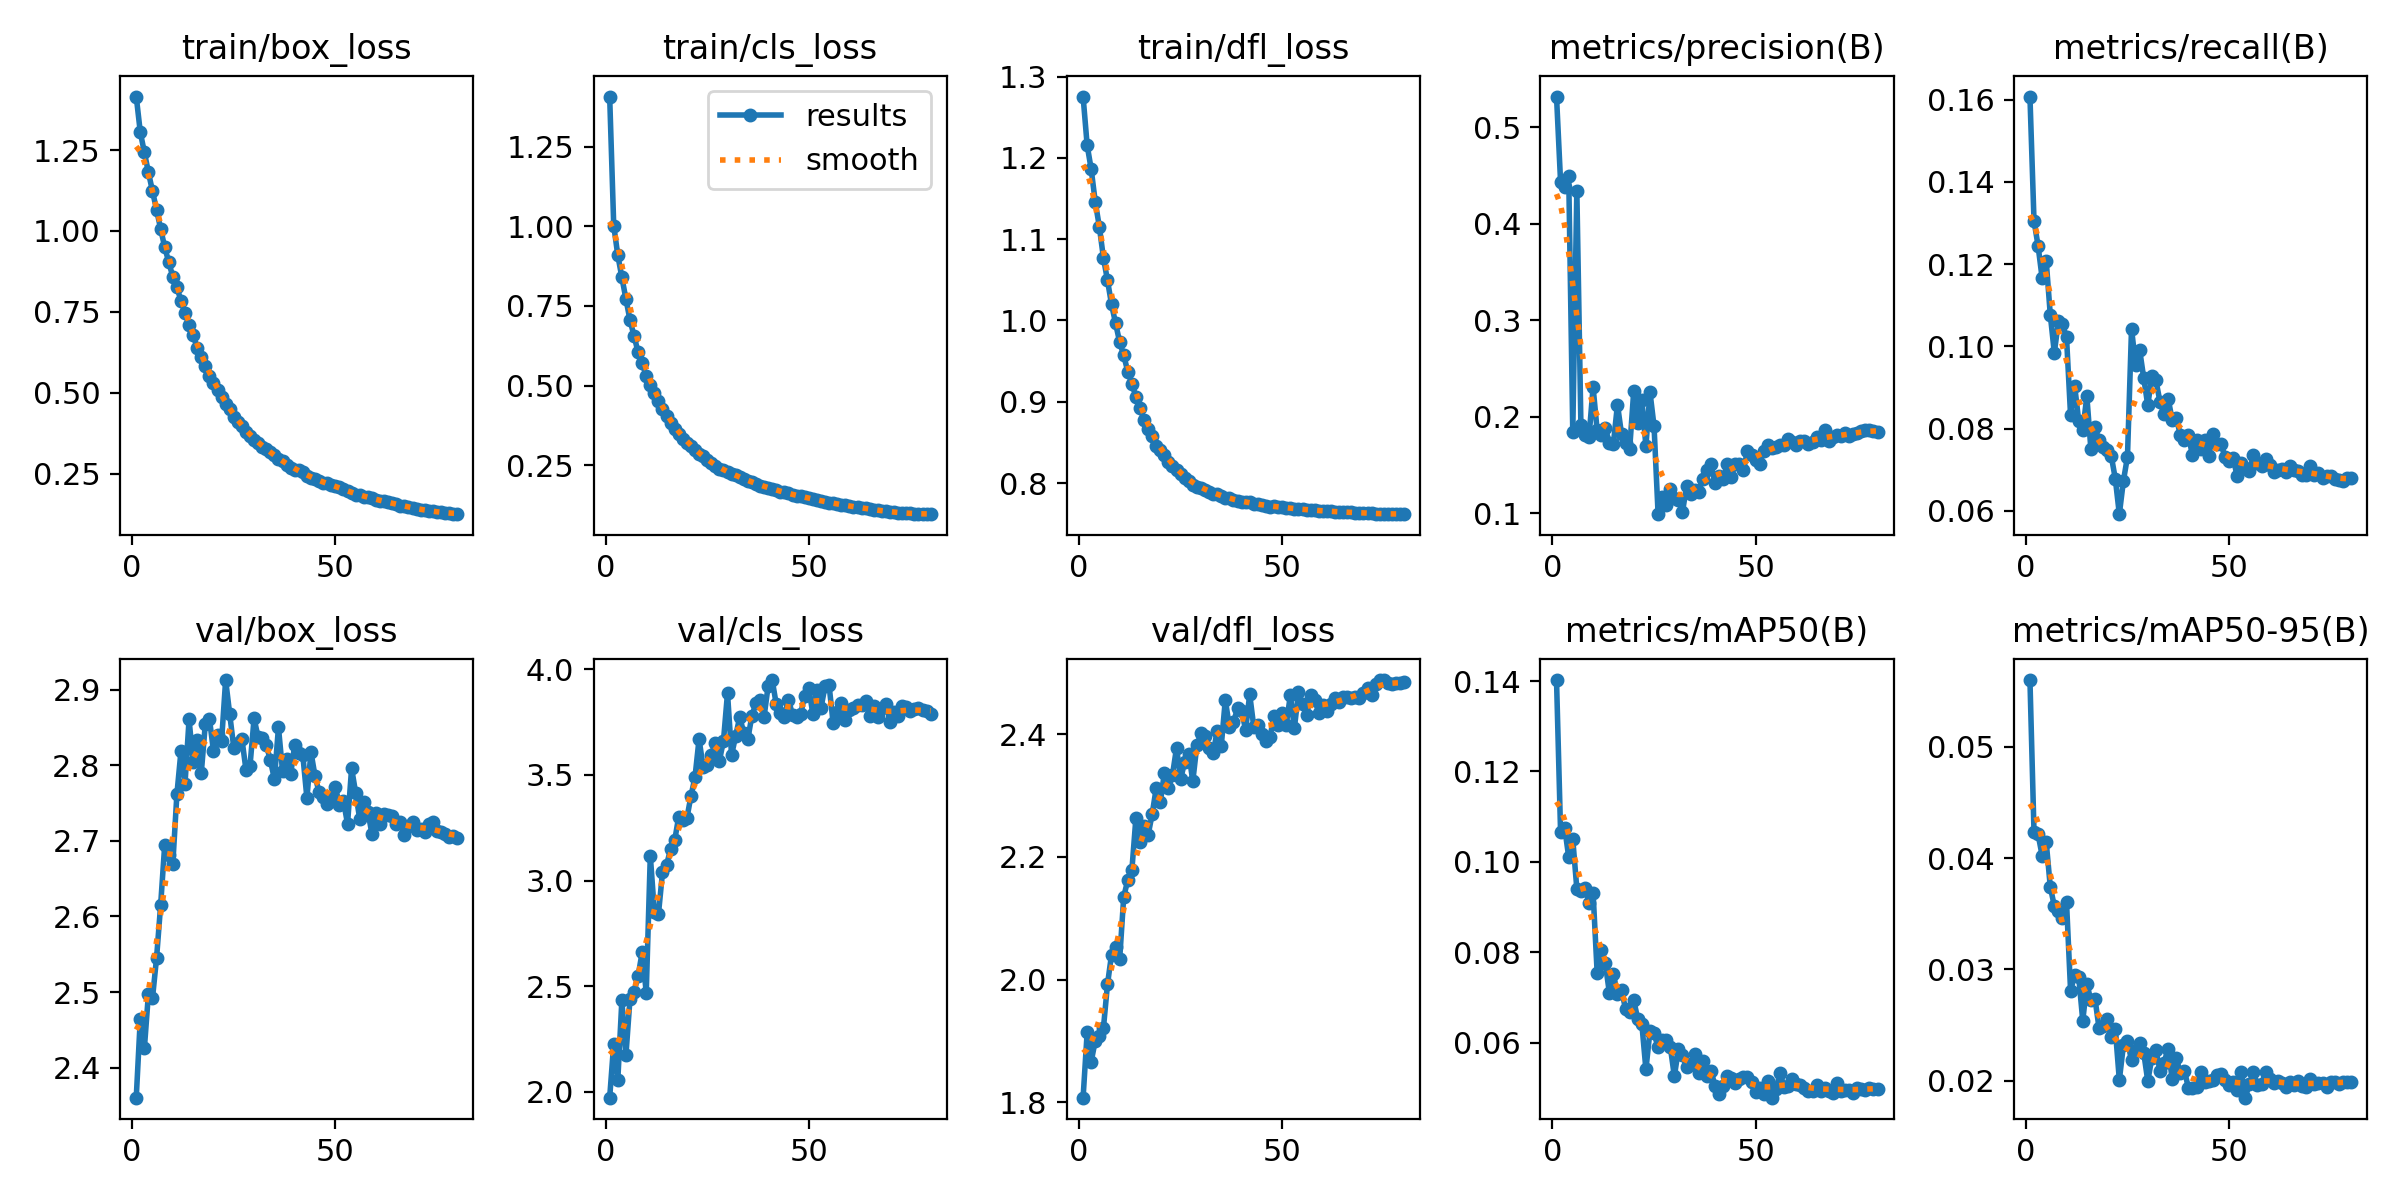
\includegraphics[width=0.48\textwidth]{runs/yolo/model1_split1_overfit/results.png}
    \hfill
    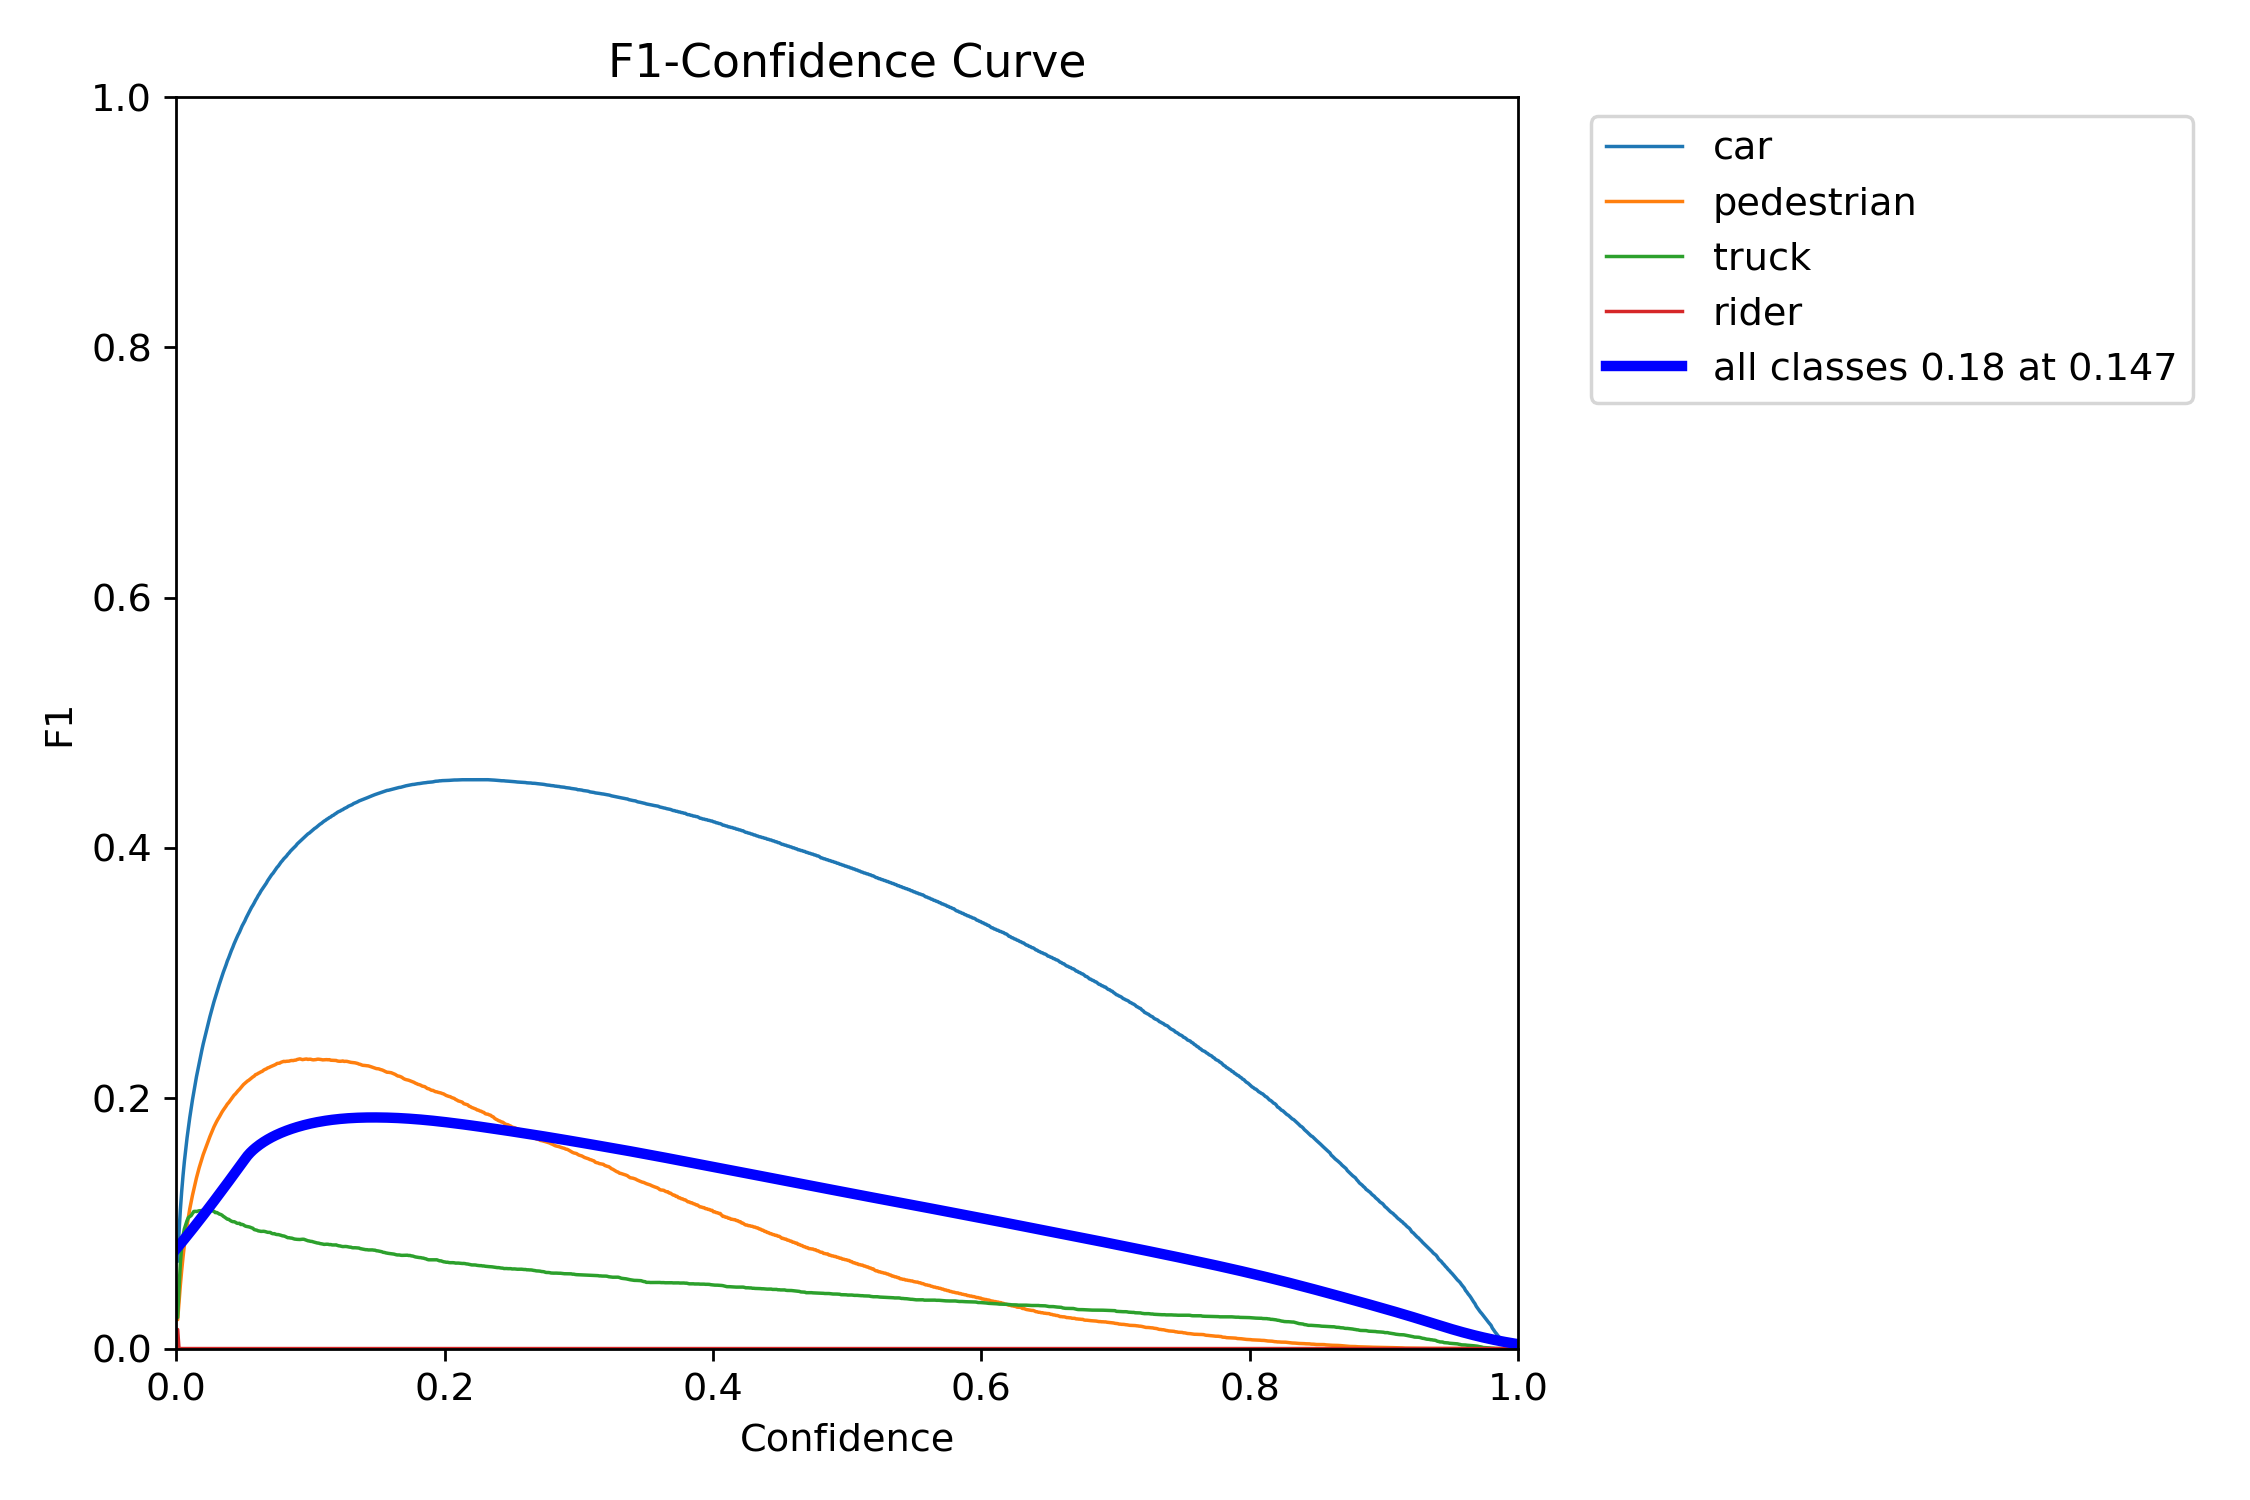
\includegraphics[width=0.48\textwidth]{runs/yolo/model1_split1_overfit/BoxF1_curve.png}
    
    \vspace{0.2cm}
    {\small \textbf{Left:} Overall training curves. \textbf{Right:} F1-Score progression.}
\end{frame}

% --- Slide 8: MODEL1 Metrics ---
\begin{frame}{MODEL1: Confusion Matrix and Predictions}
    \centering
    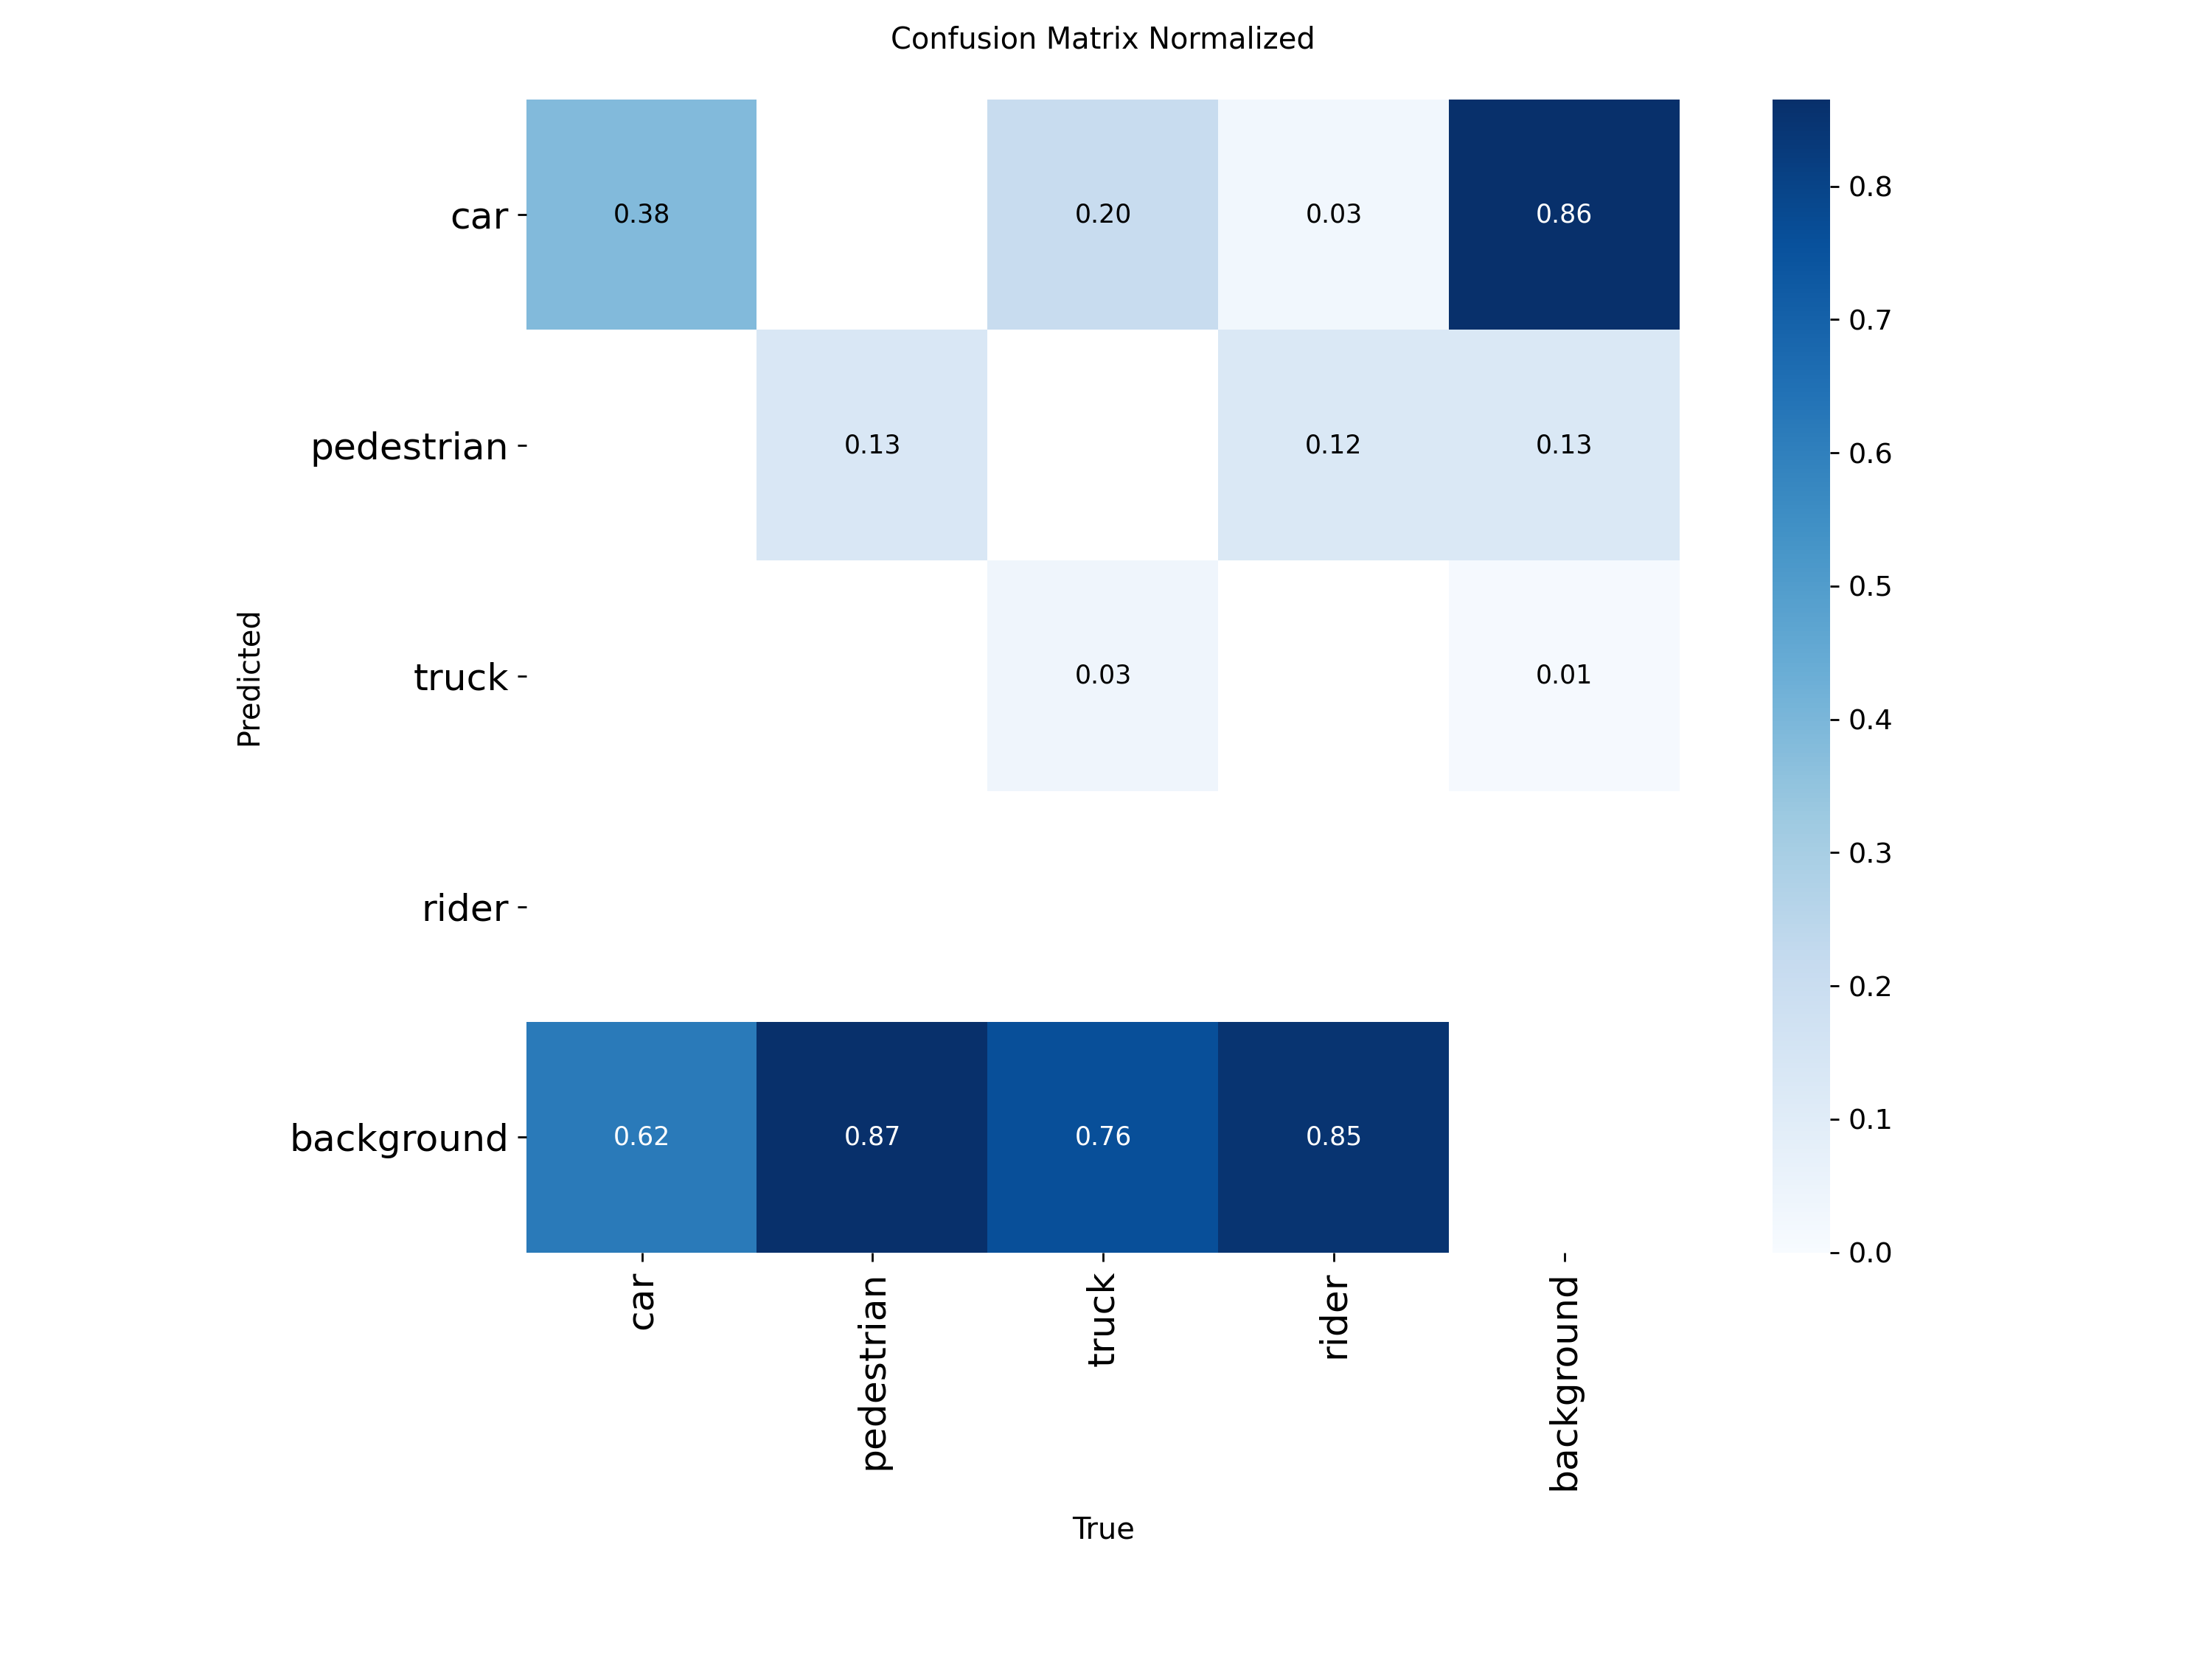
\includegraphics[width=0.48\textwidth]{runs/yolo/model1_split1_overfit/confusion_matrix_normalized.png}
    \hfill
    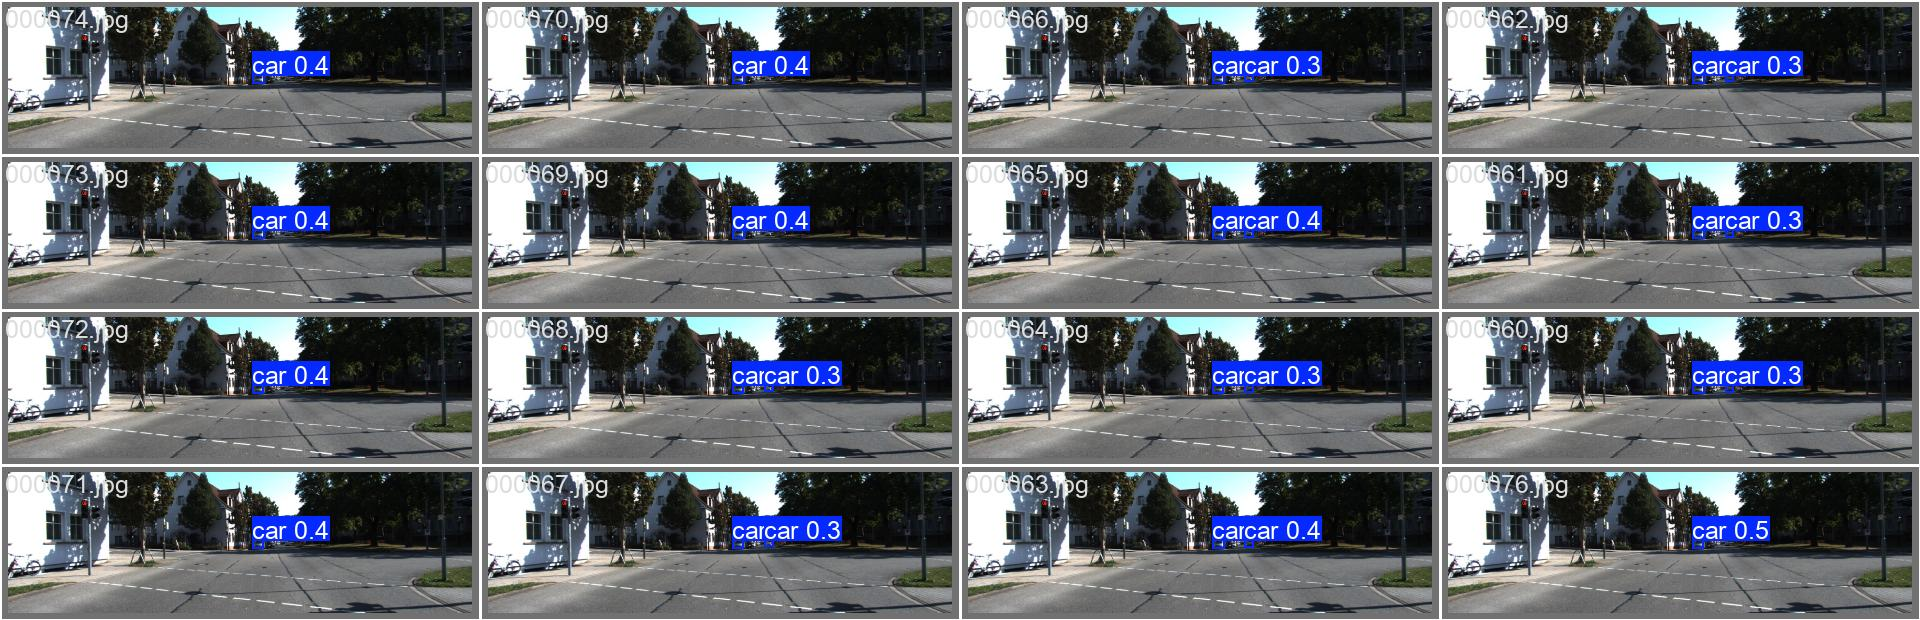
\includegraphics[width=0.48\textwidth]{runs/yolo/model1_split1_overfit/val_batch0_pred.jpg}
    
    \vspace{0.2cm}
    {\small \textbf{Left:} Normalized confusion matrix. \textbf{Right:} Predictions on validation data.}
\end{frame}

% --- Slide 9: MODEL1 Analysis ---
\begin{frame}{MODEL1: Key Observations}
    \textbf{Severe Overfitting Evidence:}
    \begin{itemize}
        \item \textbf{Train Loss:} 1.42 (epoch 1) $\rightarrow$ 0.21 (epoch 49)
        \item \textbf{Val Loss:} 2.75--2.91 (diverges significantly from train loss)
        \item \textbf{mAP50 Gap:} Train 13.5\% vs. Val 5.2\% (3$\times$ worse!)
        \item \textbf{Train-Val Gap:} 8.3 mAP percentage points
    \end{itemize}

    \vspace{0.3cm}
    \textbf{Challenges and Interesting Issues:}
    \begin{itemize}
        \item Tiny dataset (2\%) with only 26K training boxes causes severe memorization
        \item Zero augmentation prevents model from seeing data variations
        \item Model memorizes rather than learns generalizable features
        \item Per-class performance highly uneven (confusion matrix shows class bias)
    \end{itemize}

    \vspace{0.3cm}
    \textbf{Conclusions and Experiences:}
    \begin{itemize}
        \item Quantifies how severe overfitting can be even with powerful pre-trained models
        \item Train-Val gap is a diagnostic tool for detecting overfitting
        \item Full dataset (MODEL2) should eliminate this gap
    \end{itemize}
\end{frame}

% --- Slide 10: MODEL2 Overview ---
\begin{frame}{MODEL2 (SPLIT2): Full Dataset Training}
    \textbf{Objective:} Train on complete dataset with standard regularization.
    
    \vspace{0.3cm}
    \textbf{Configuration:}
    \begin{itemize}
        \item \textbf{Data:} 100\% of SPLIT2/TRAIN ($\approx$ 1.3M instances)
        \item \textbf{Augmentation:} \textbf{Enabled} (mosaic, mixup, color shifts, shear, translate)
        \item \textbf{Epochs:} 20
        \item \textbf{Batch Size:} 12
        \item \textbf{Image Resolution:} 960 × 960 px
        \item \textbf{Early Stopping:} Yes (patience=20)
        \item \textbf{Workers:} 8 (parallel data loading)
    \end{itemize}

    \vspace{0.3cm}
    \textbf{Expected Outcome:}
    \begin{itemize}
        \item Train and Val losses track closely (minimal divergence)
        \item Model learns generalizable features
        \item Val performance $\approx$ 80--90\% of train performance
    \end{itemize}
\end{frame}

% --- Slide 11: MODEL2 Results - Loss Curves ---
\begin{frame}{MODEL2: Training Progress}
    \centering
    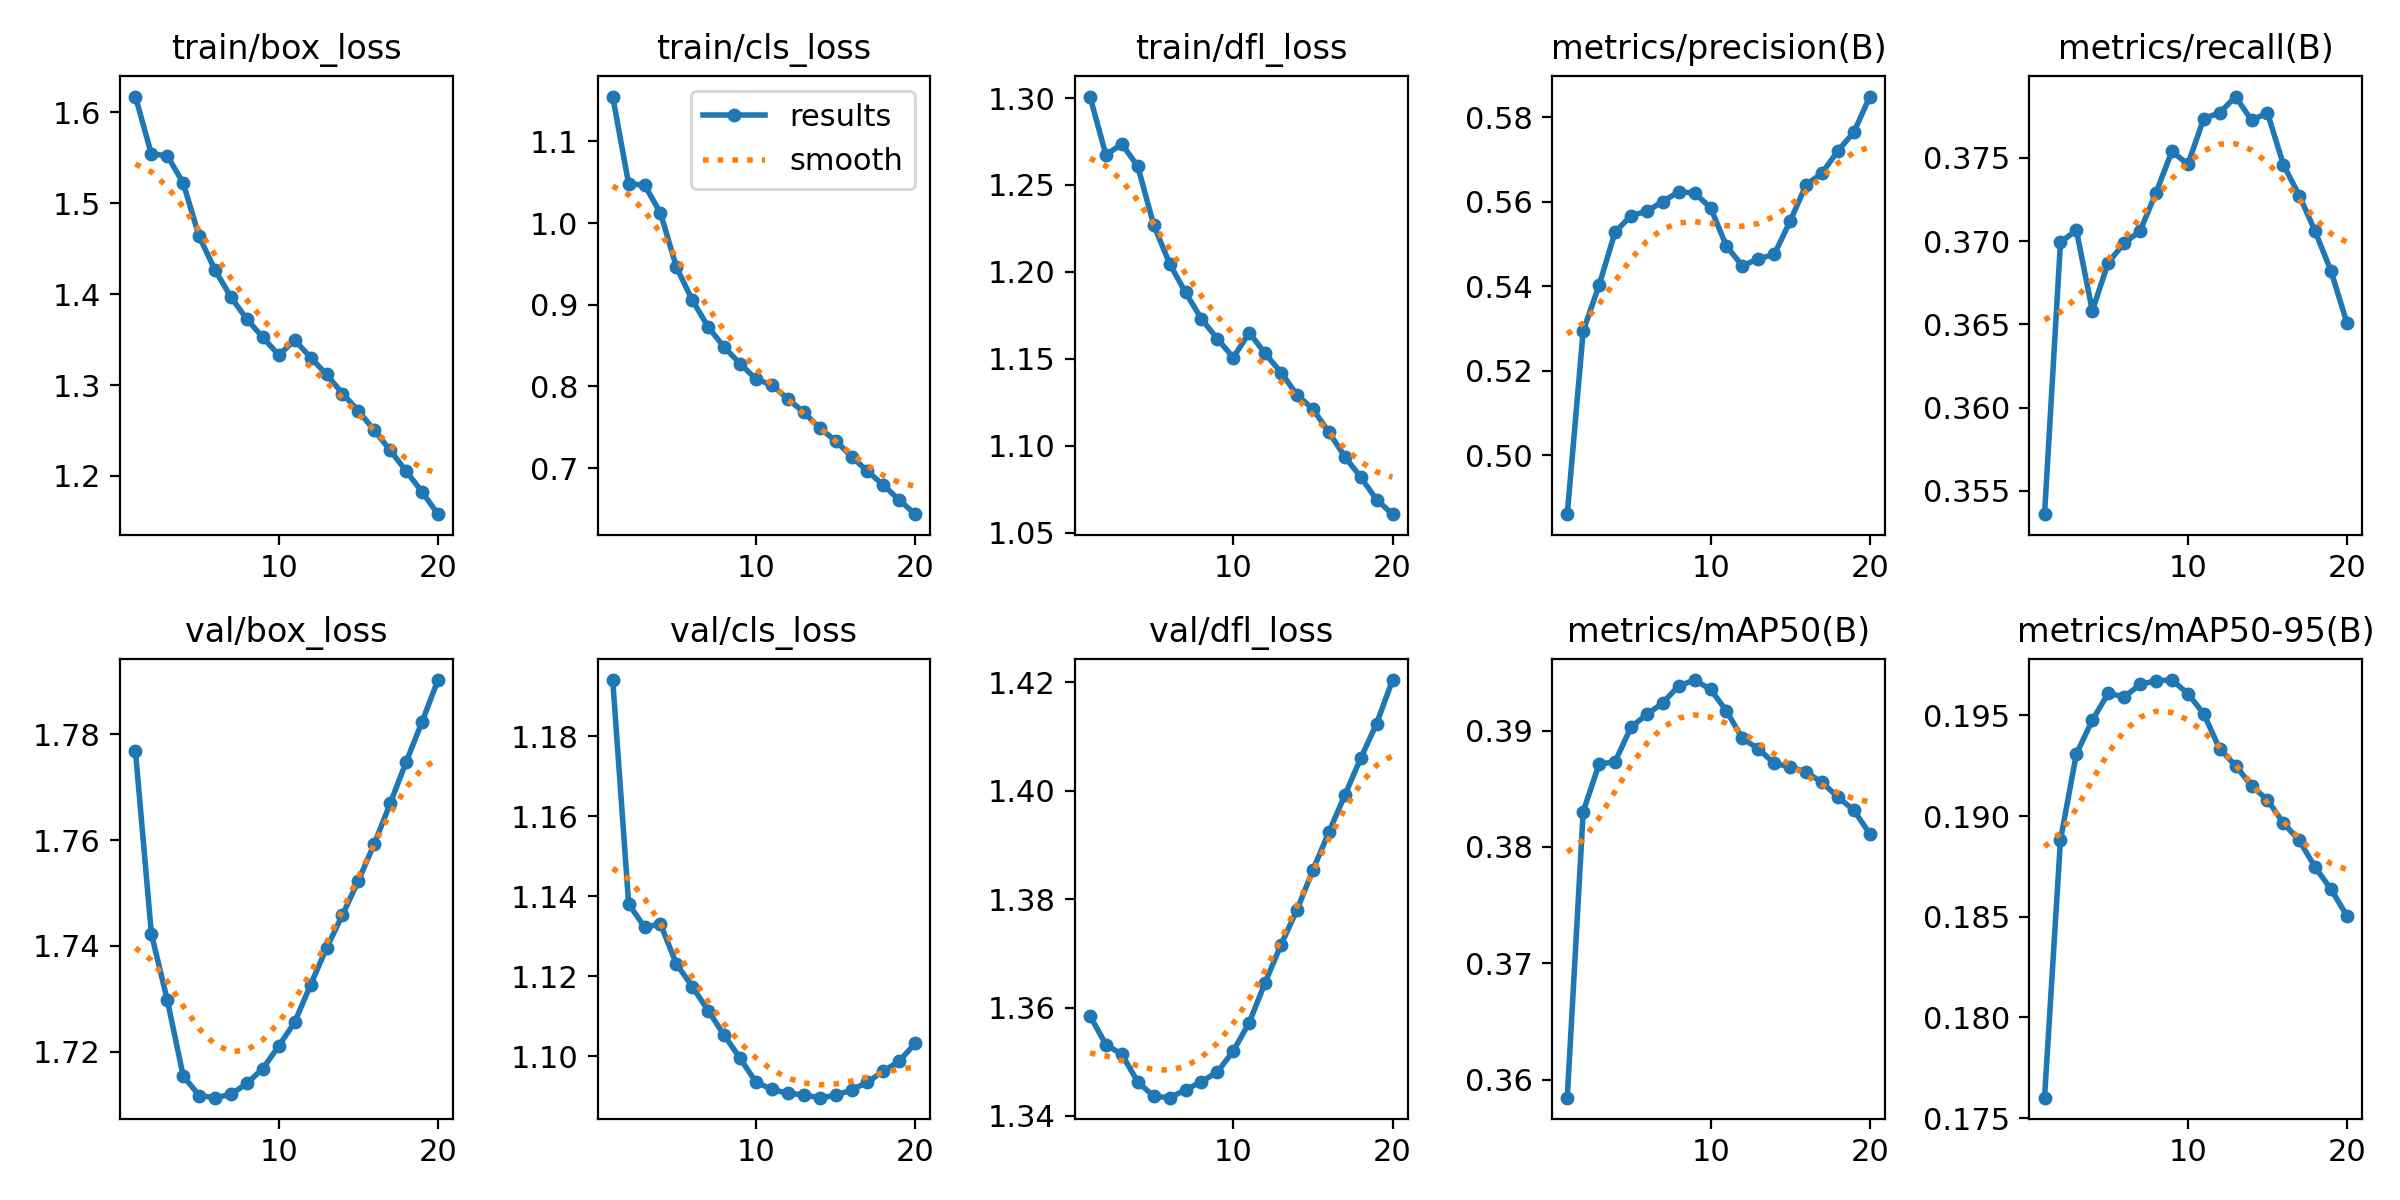
\includegraphics[width=0.48\textwidth]{runs/yolo/model2_split2-4/results.png}
    \hfill
    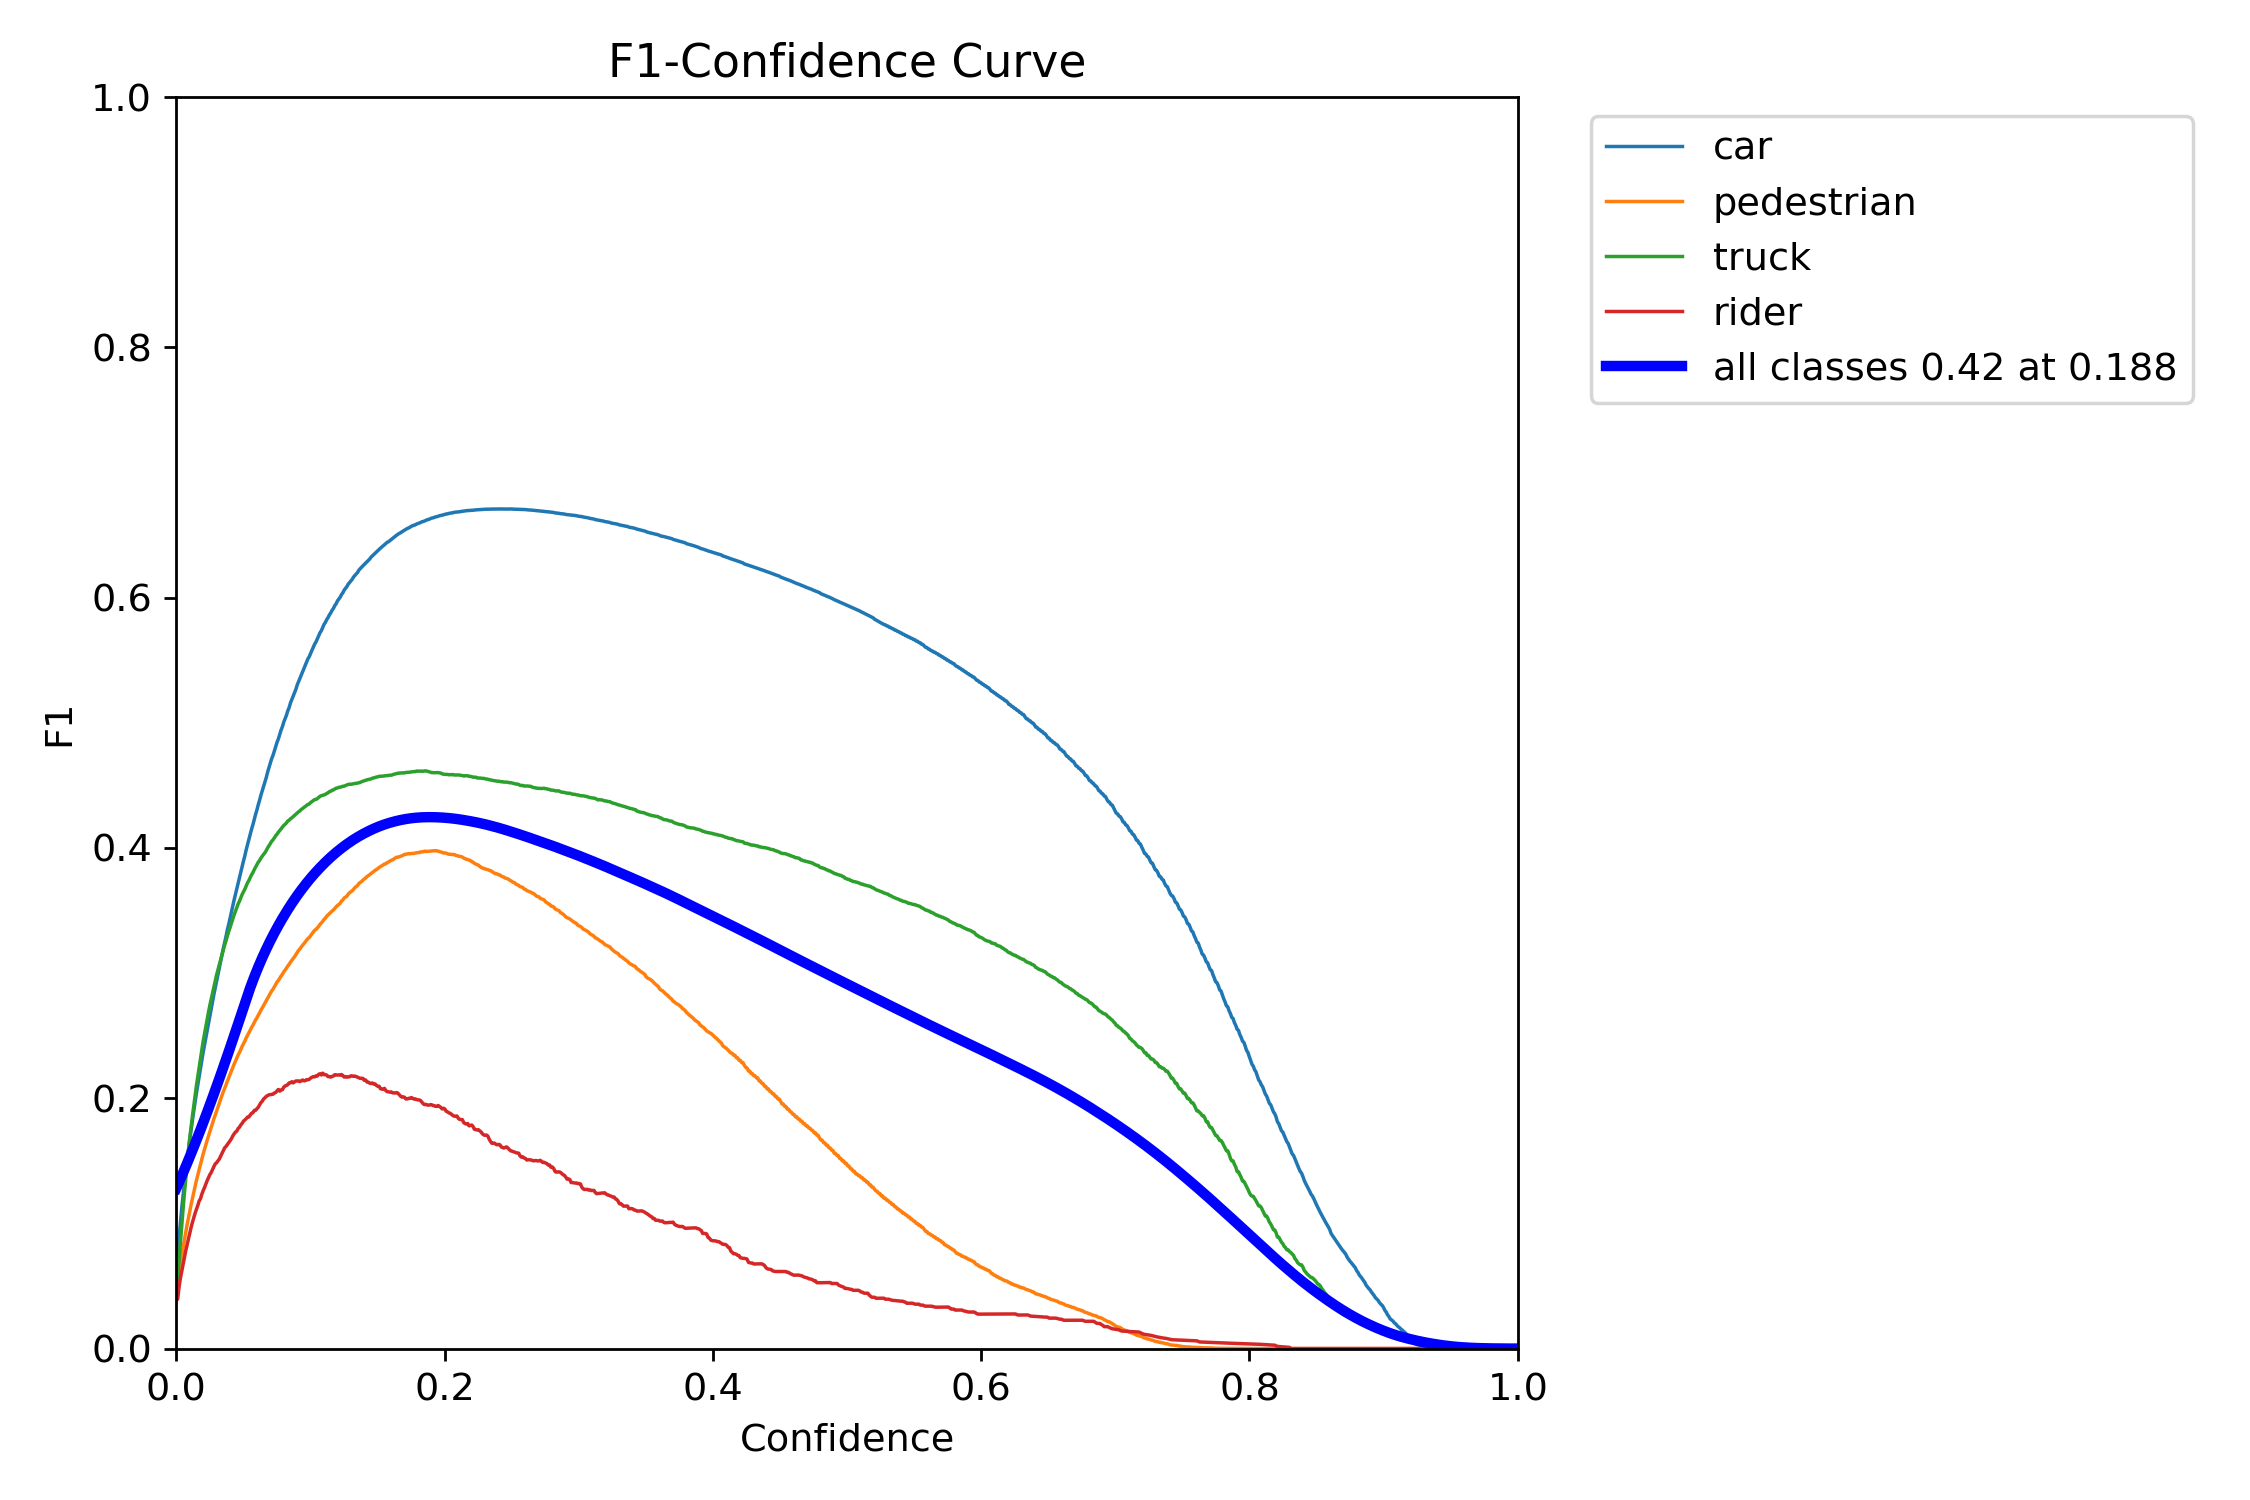
\includegraphics[width=0.48\textwidth]{runs/yolo/model2_split2-4/BoxF1_curve.png}
    
    \vspace{0.2cm}
    {\small \textbf{Left:} Overall training curves. \textbf{Right:} F1-Score progression.}
\end{frame}

% --- Slide 12: MODEL2 Metrics ---
\begin{frame}{MODEL2: Confusion Matrix and Predictions}
    \centering
    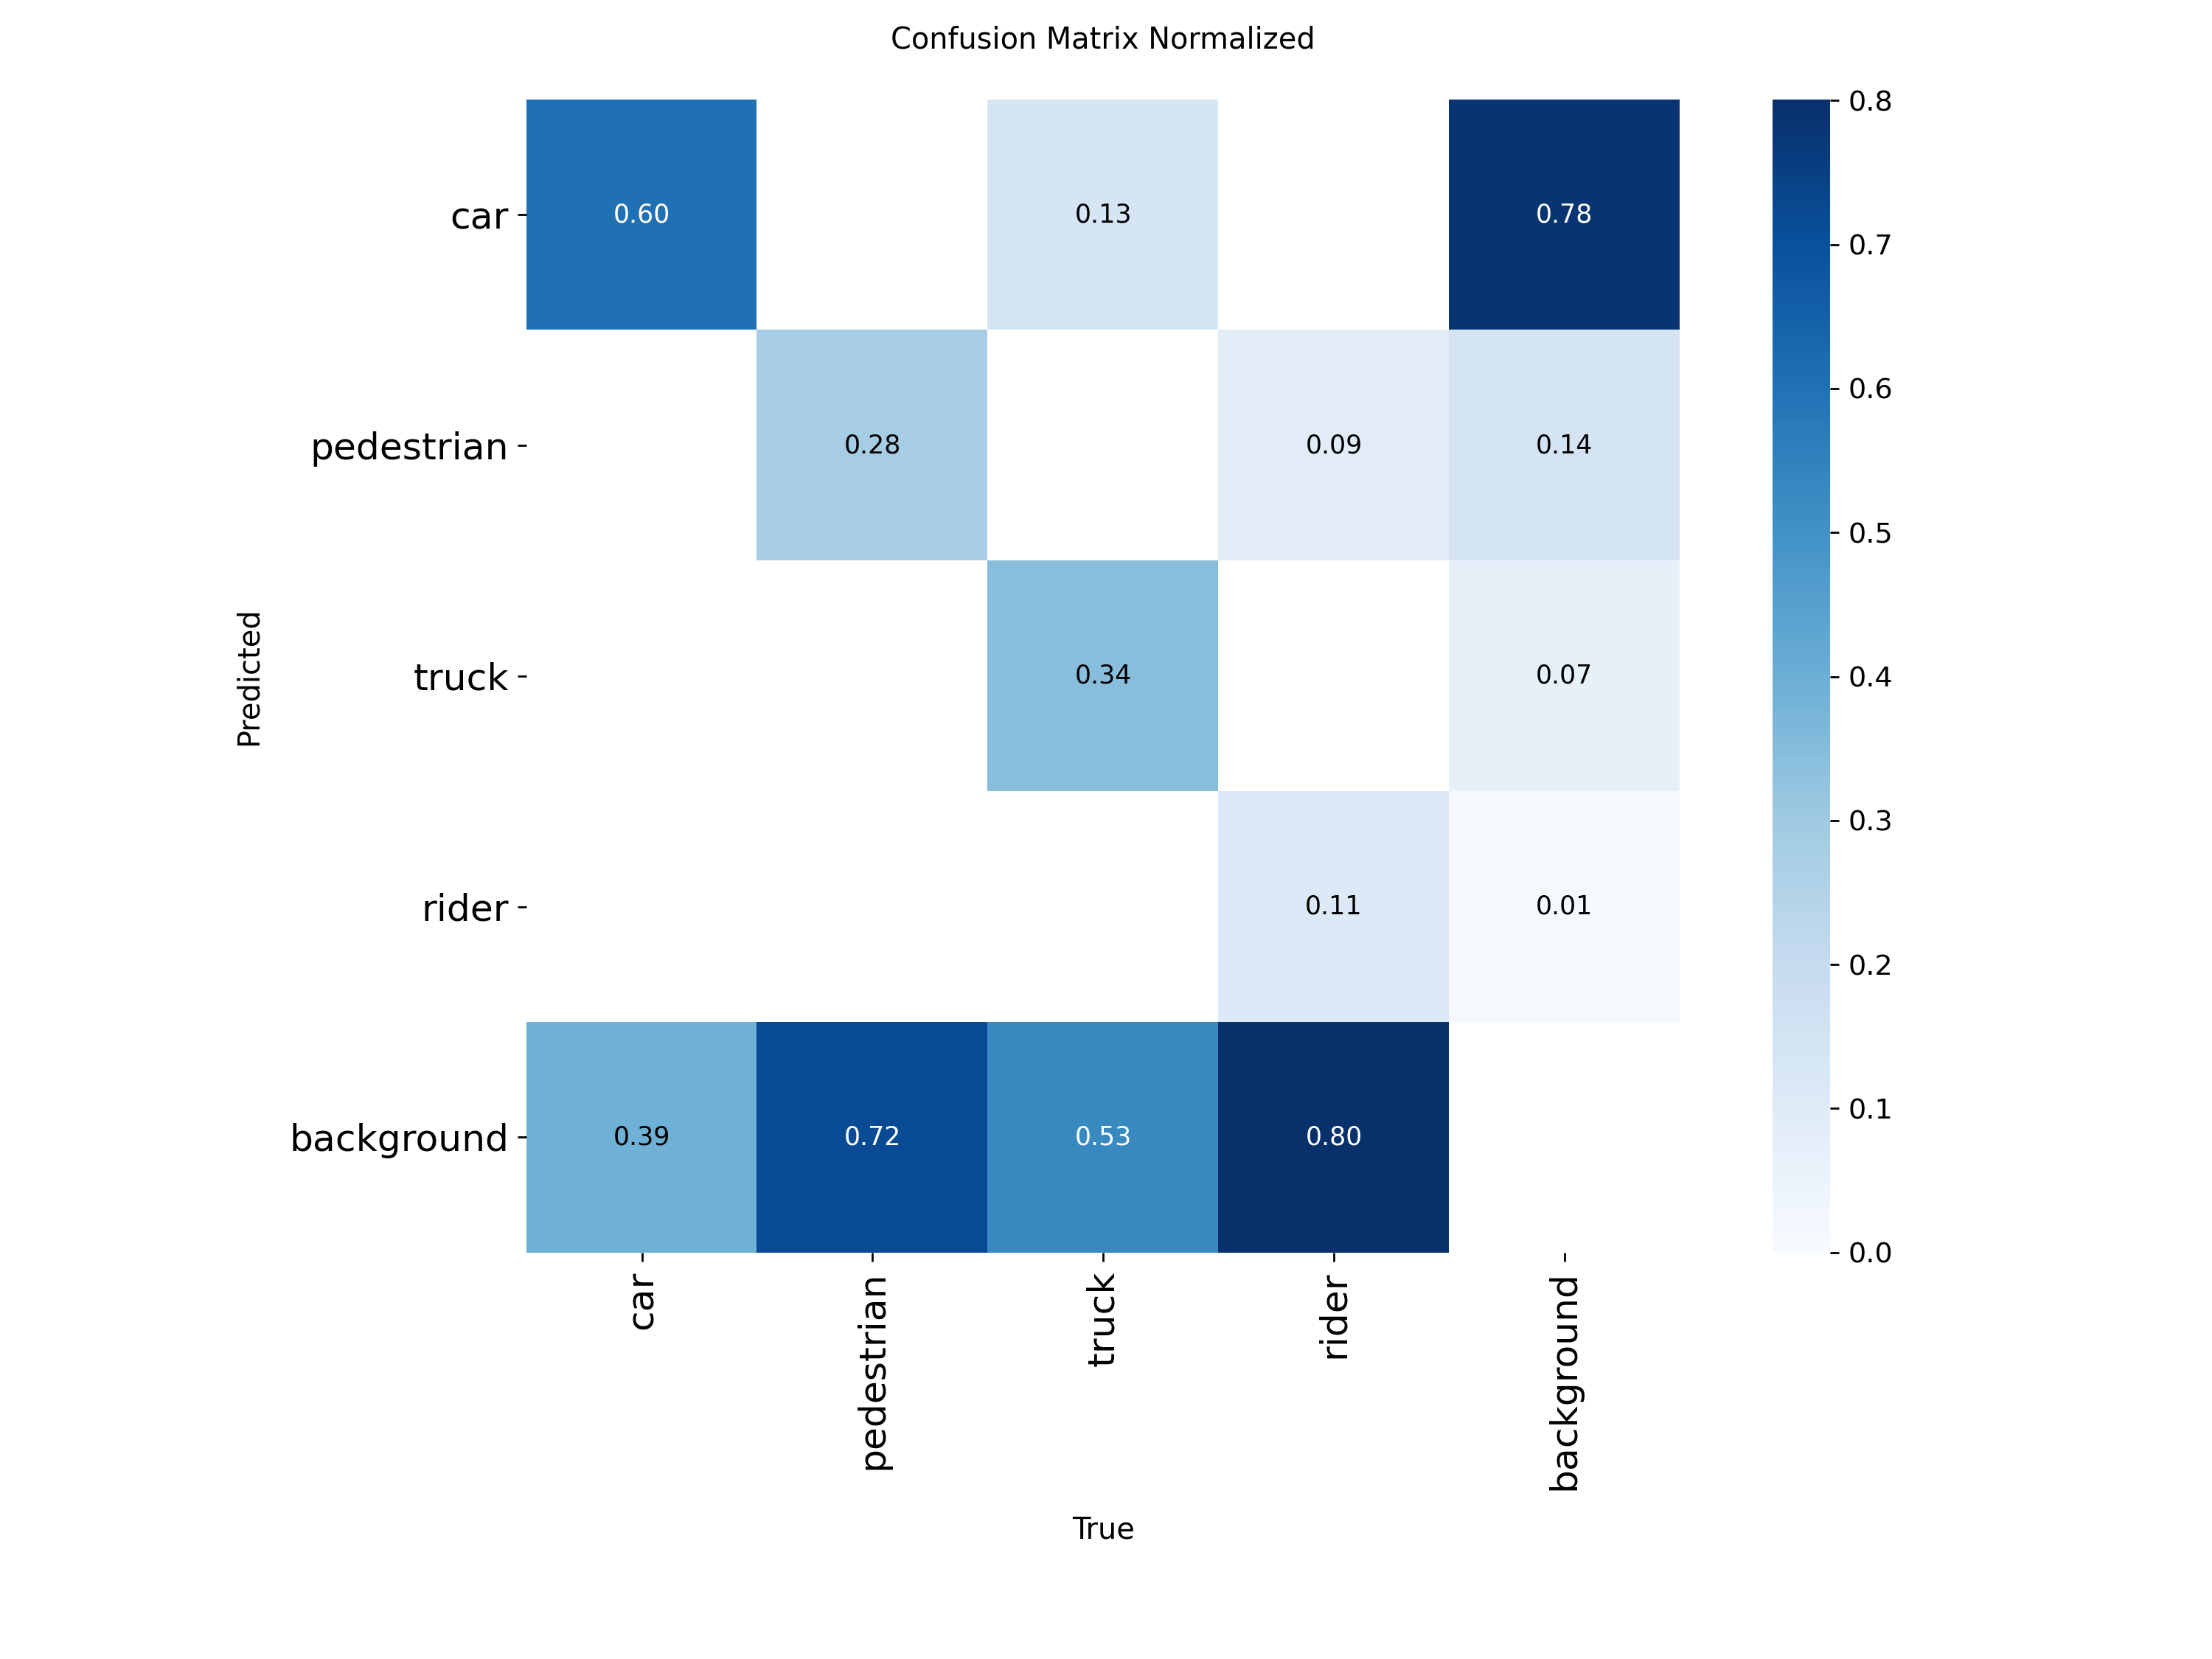
\includegraphics[width=0.48\textwidth]{runs/yolo/model2_split2-4/confusion_matrix_normalized.png}
    \hfill
    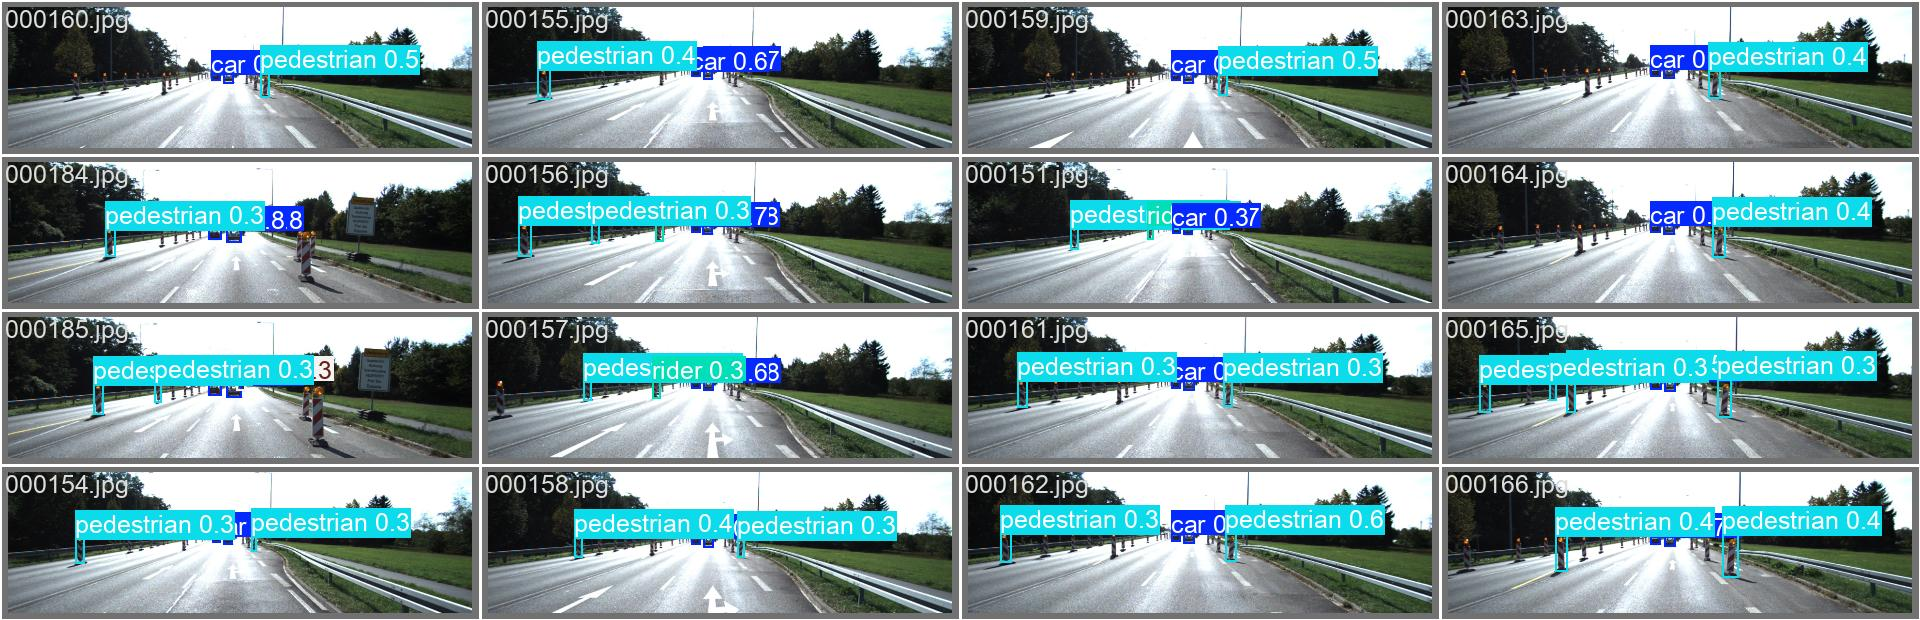
\includegraphics[width=0.48\textwidth]{runs/yolo/model2_split2-4/val_batch0_pred.jpg}
    
    \vspace{0.2cm}
    {\small \textbf{Left:} Normalized confusion matrix. \textbf{Right:} Predictions on validation data.}
\end{frame}

% --- Slide 13: MODEL2 Analysis ---
\begin{frame}{MODEL2: Key Observations}
    \textbf{Excellent Generalization:}
    \begin{itemize}
        \item \textbf{Train Loss:} 1.62 $\rightarrow$ 1.16 (epoch 20)
        \item \textbf{Val Loss:} 1.78 $\rightarrow$ 1.79 (remains stable!)
        \item \textbf{Train-Val Gap:} Only 0.63 (minimal divergence)
        \item \textbf{mAP50:} Train $\approx$ 58.4\%, Val $\approx$ 58.1\% (nearly identical!)
    \end{itemize}

    \vspace{0.3cm}
    \textbf{Challenges and Interesting Issues:}
    \begin{itemize}
        \item Minority classes (rider) remain challenging: $\sim$50\% lower recall than cars
        \item Early stopping at epoch 20 suggests convergence reached
        \item Class imbalance persists despite augmentation and regularization
    \end{itemize}

    \vspace{0.3cm}
    \textbf{Conclusions and Experiences:}
    \begin{itemize}
        \item Large training set (1.3M instances) prevents memorization
        \item Data augmentation forces learning of robust features
        \item Proper validation set (separate videos) provides honest evaluation
        \item This is the model recommended for deployment
    \end{itemize}
\end{frame}

% --- Slide 14: MODEL3 Overview ---
\begin{frame}{MODEL3 (SPLIT3): Data Leakage Demonstration}
    \textbf{Objective:} Demonstrate impact of data leakage on validation metrics.
    
    \vspace{0.3cm}
    \textbf{Configuration:}
    \begin{itemize}
        \item \textbf{Data:} 100\% of SPLIT3/TRAIN ($\approx$ 1.3M instances)
        \item \textbf{Validation Set:} \textbf{Drawn from SPLIT3/TRAIN} (20\% of training set)
        \item \textbf{Key Difference:} VAL contains frames from videos ALREADY in TRAIN
        \item \textbf{Augmentation:} Same as MODEL2
        \item \textbf{Other parameters:} Identical to MODEL2
    \end{itemize}

    \vspace{0.3cm}
    \textbf{The Leak Mechanism:}
    \begin{itemize}
        \item \textbf{MODEL2:} VAL set from completely separate videos (no leakage)
        \item \textbf{MODEL3:} VAL set from same videos as TRAIN (80\% overlap)
        \item Result: Model has essentially already seen the validation data
    \end{itemize}
\end{frame}

% --- Slide 15: MODEL3 Results - Loss Curves ---
\begin{frame}{MODEL3: Training Progress}
    \centering
    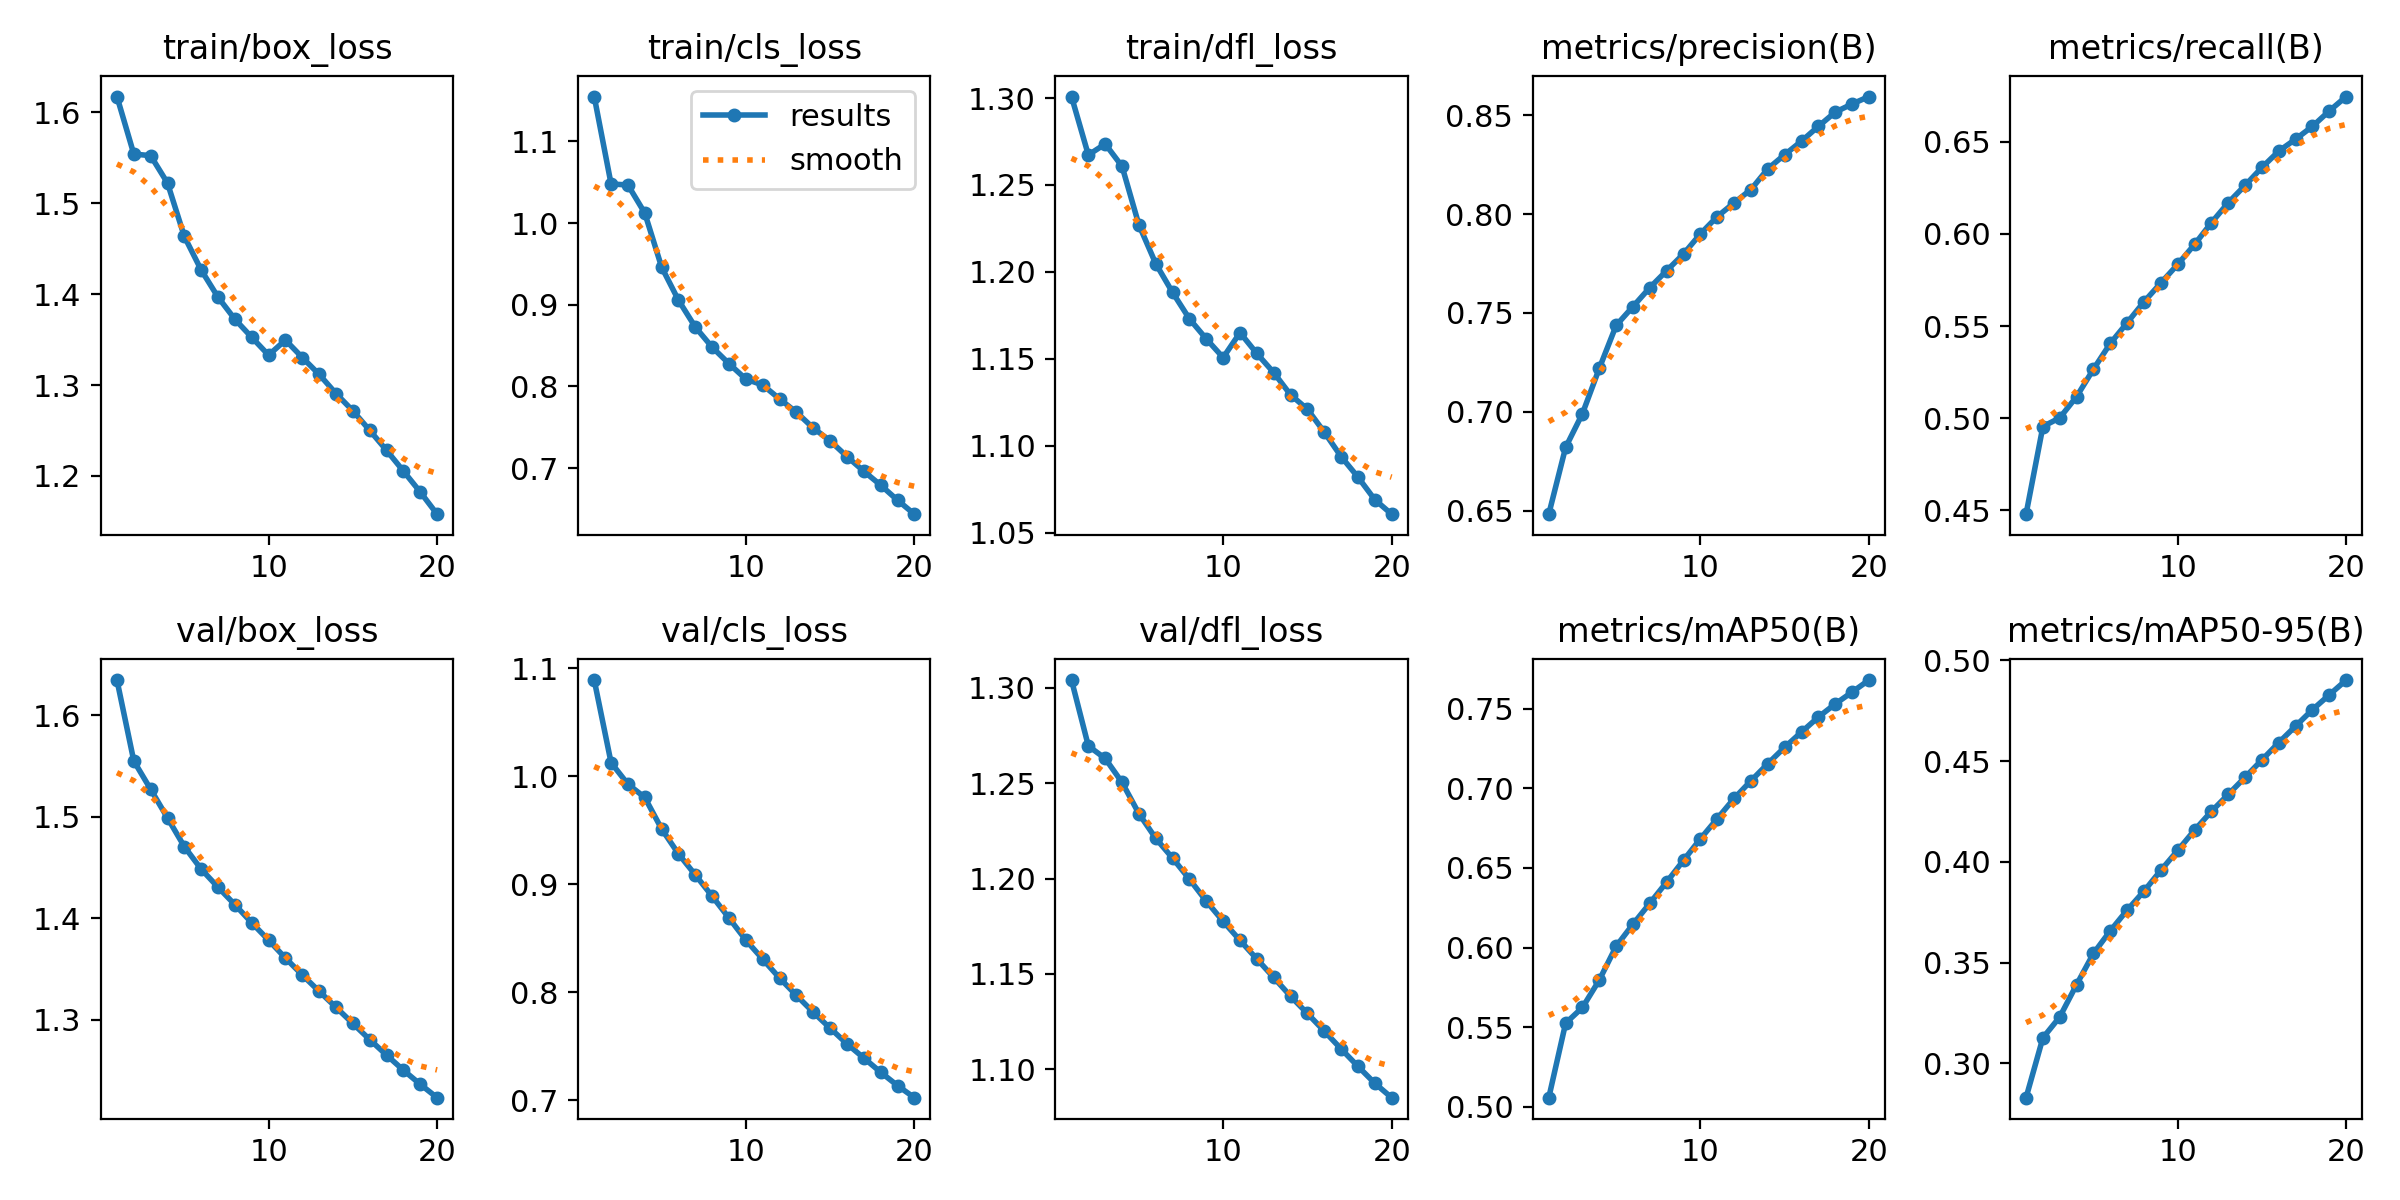
\includegraphics[width=0.48\textwidth]{runs/yolo/model3_split3/results.png}
    \hfill
    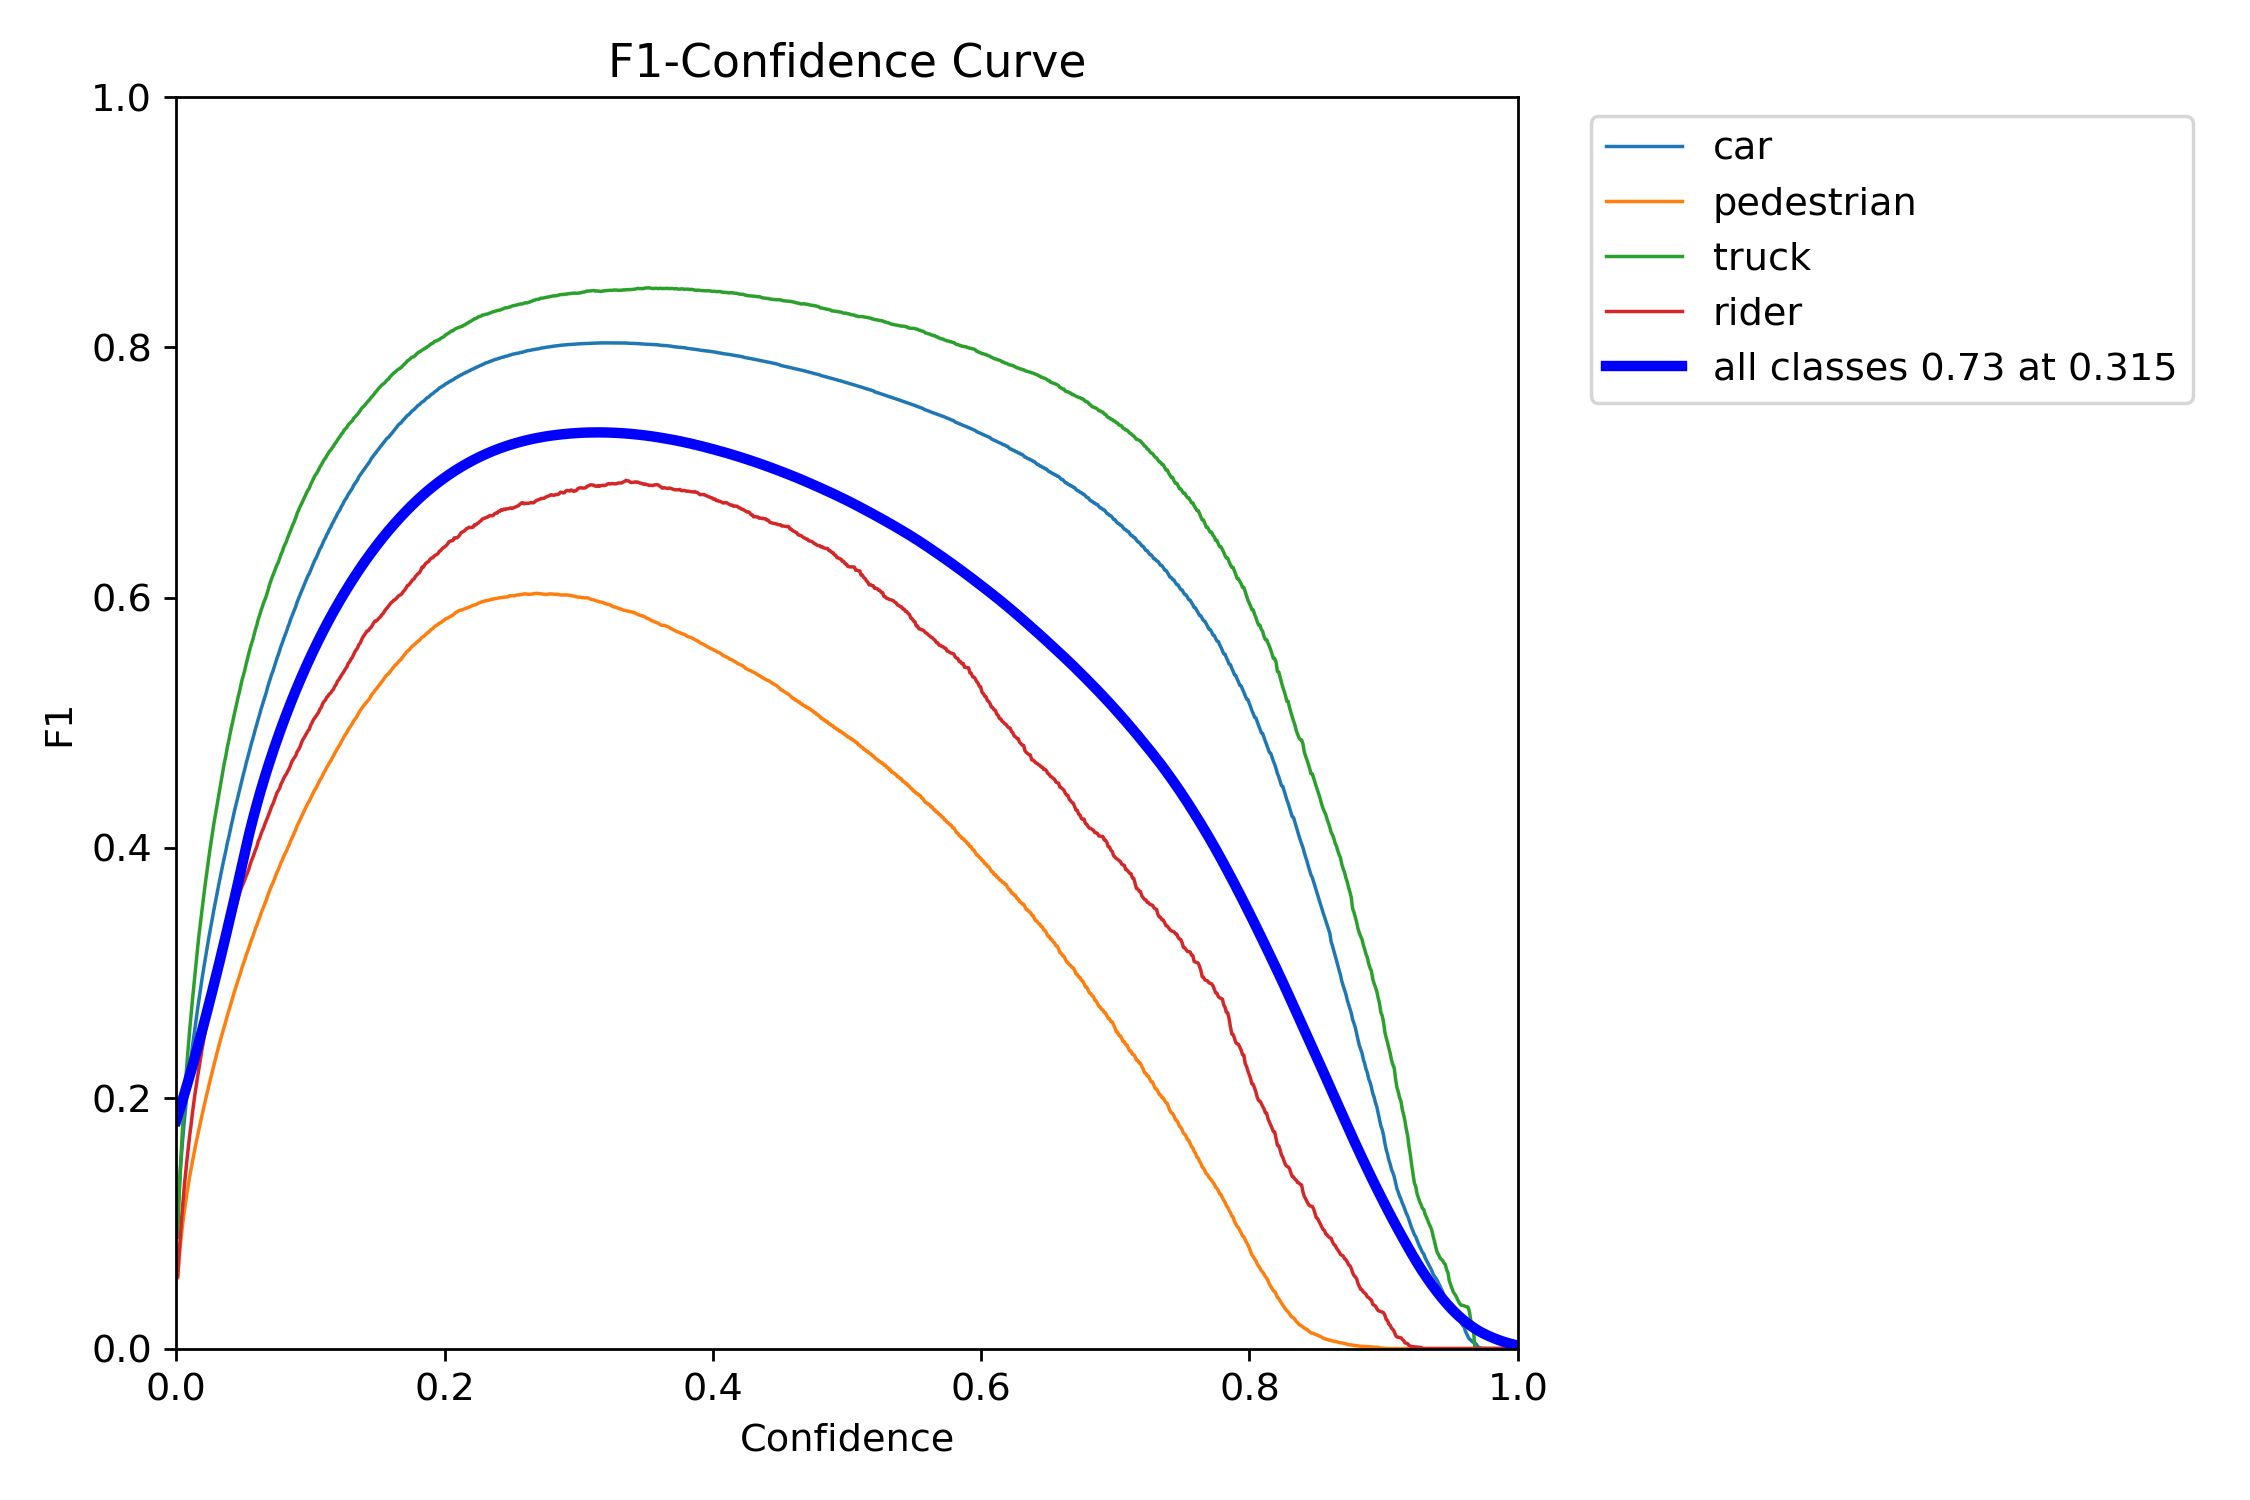
\includegraphics[width=0.48\textwidth]{runs/yolo/model3_split3/BoxF1_curve.png}
    
    \vspace{0.2cm}
    {\small \textbf{Left:} Overall training curves. \textbf{Right:} F1-Score progression.}
\end{frame}

% --- Slide 16: MODEL3 Metrics ---
\begin{frame}{MODEL3: Confusion Matrix and Predictions}
    \centering
    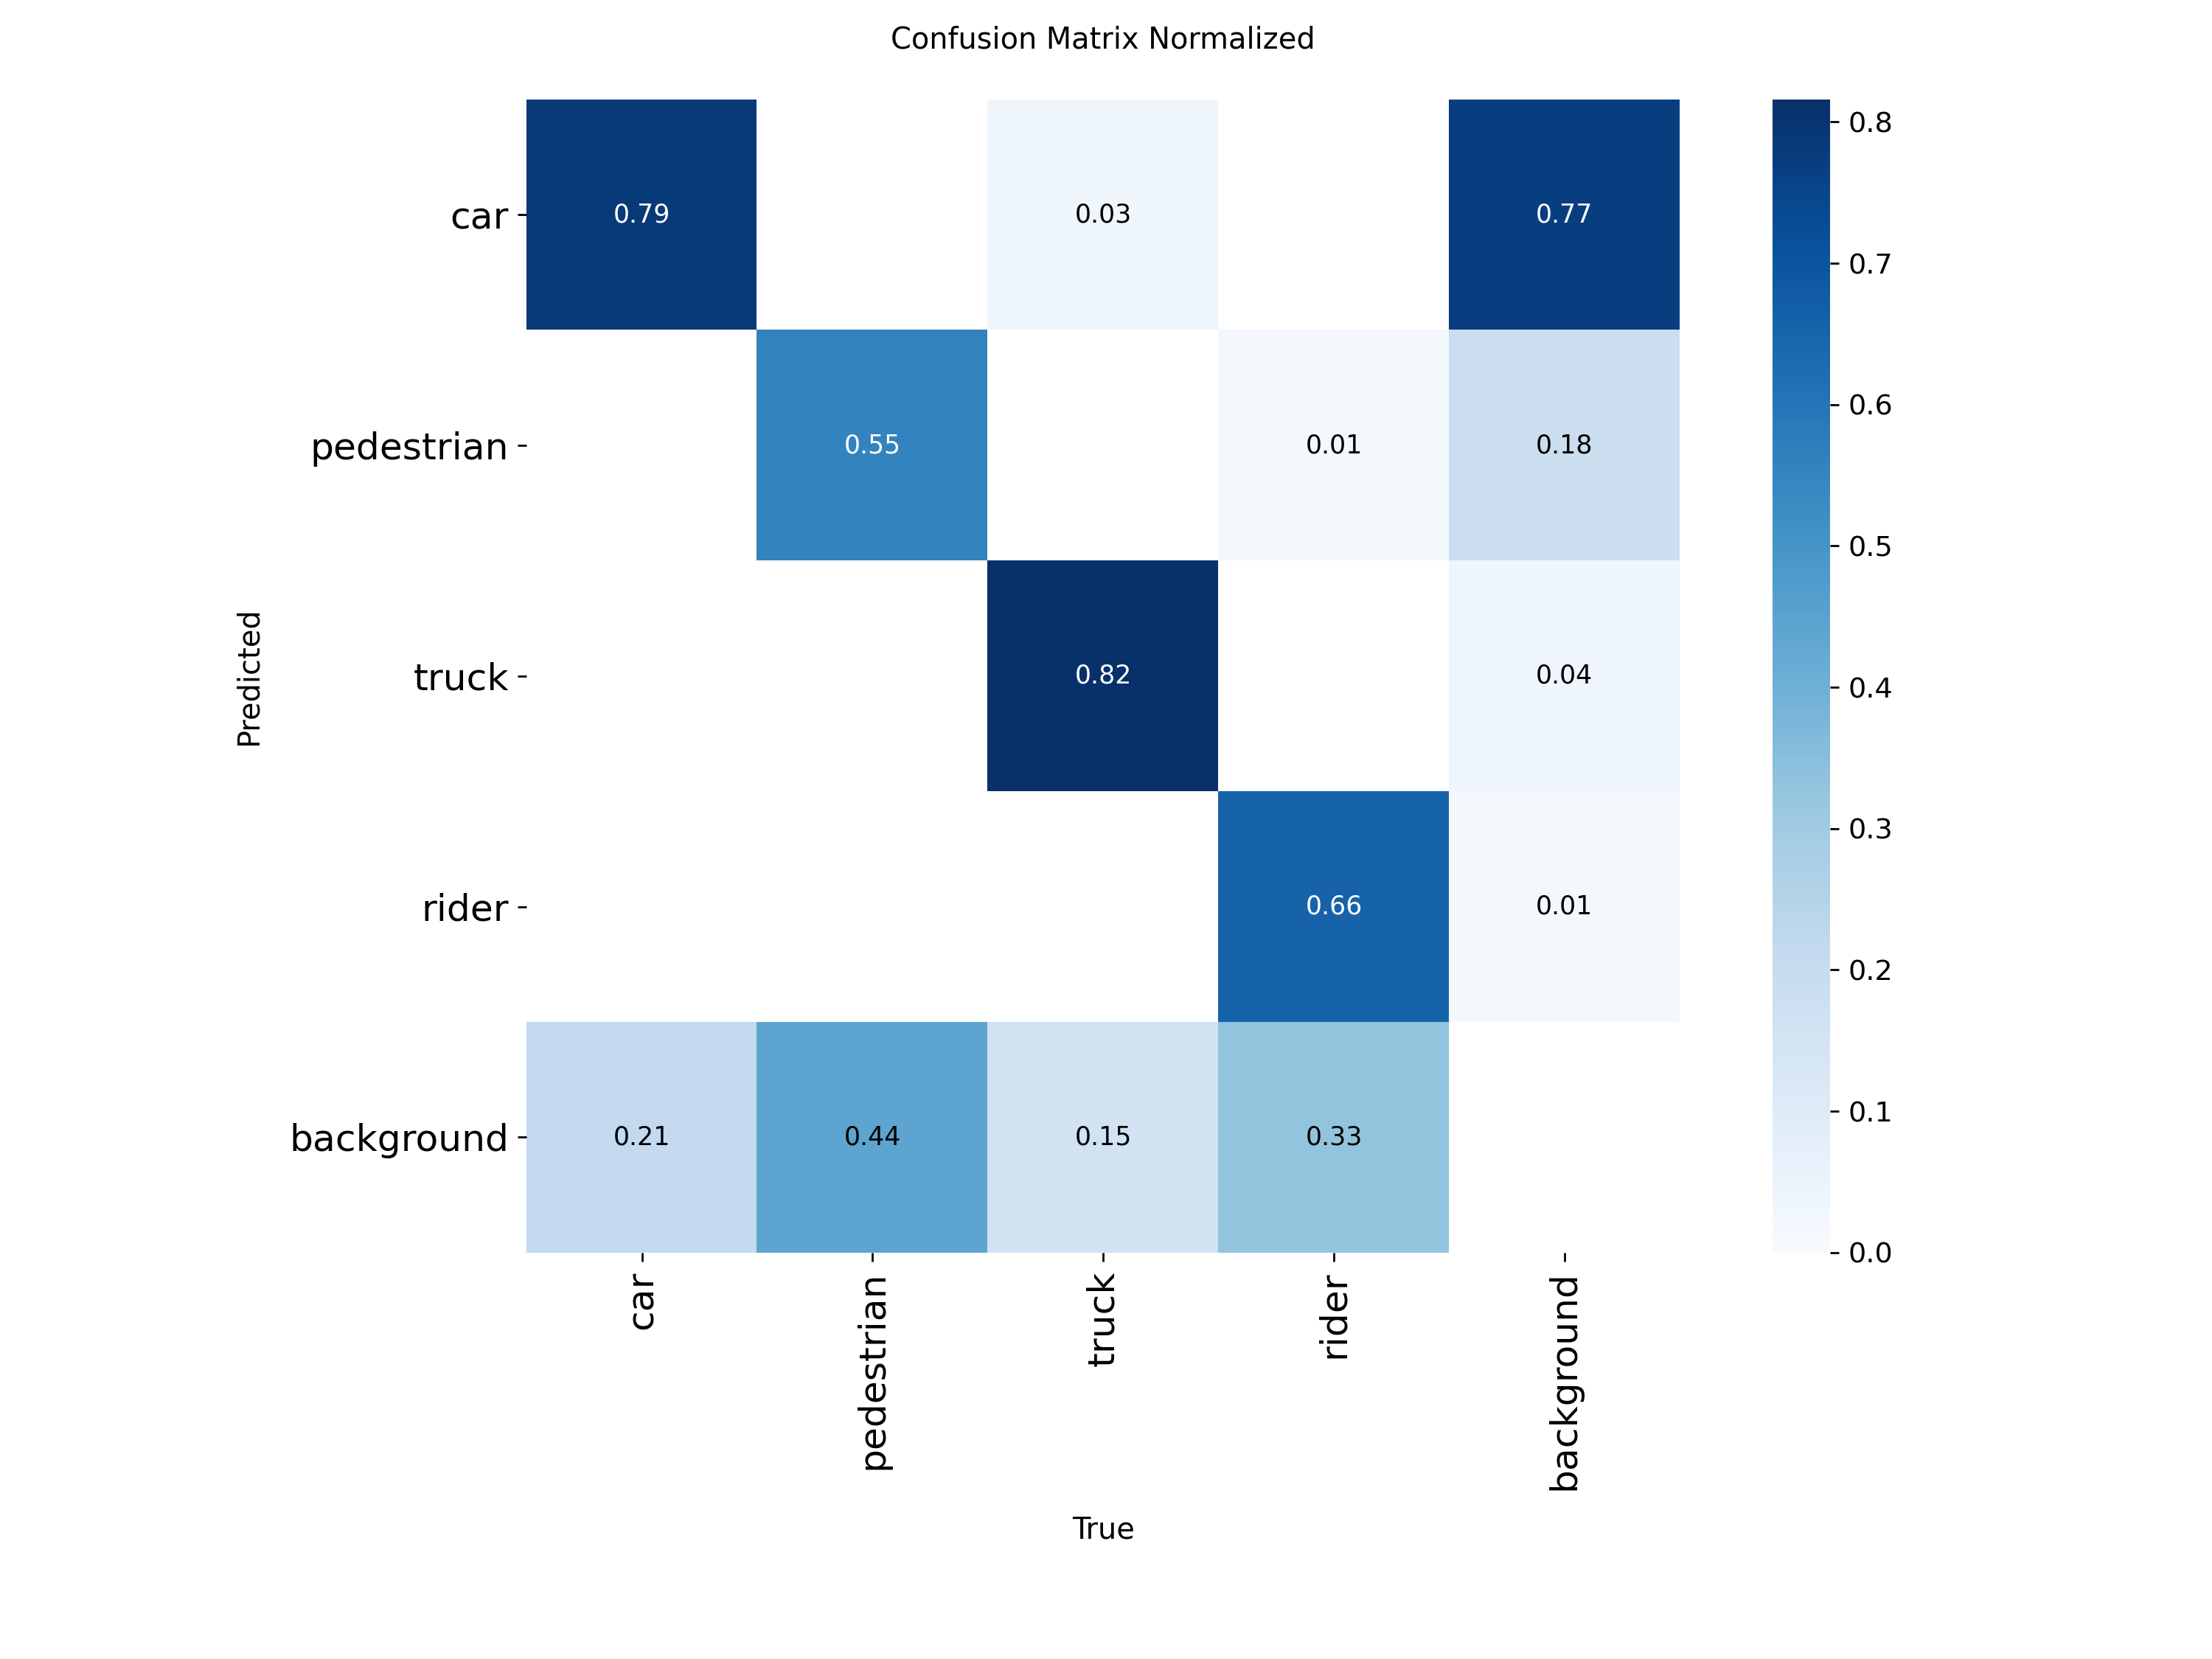
\includegraphics[width=0.48\textwidth]{runs/yolo/model3_split3/confusion_matrix_normalized.png}
    \hfill
    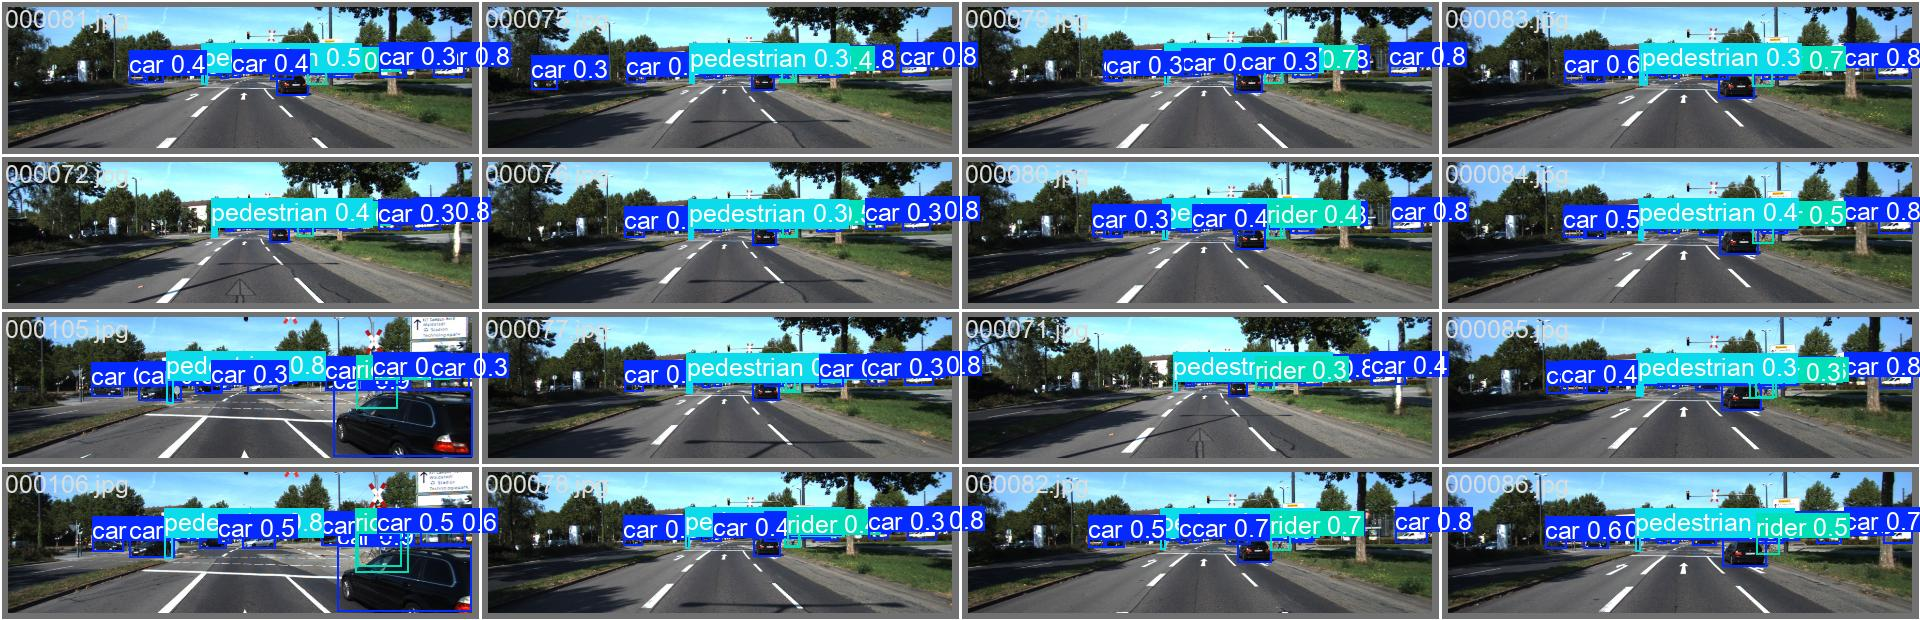
\includegraphics[width=0.48\textwidth]{runs/yolo/model3_split3/val_batch0_pred.jpg}
    
    \vspace{0.2cm}
    {\small \textbf{Left:} Normalized confusion matrix. \textbf{Right:} Predictions on validation data.}
\end{frame}

% --- Slide 17: MODEL3 Analysis - Data Leakage ---
\begin{frame}{MODEL3: Key Observations}
    \textbf{Artificially Inflated Metrics:}
    \begin{itemize}
        \item \textbf{Train Loss:} 1.62 $\rightarrow$ 1.15 (nearly identical to MODEL2)
        \item \textbf{Val Loss:} 1.77 (vs. MODEL2's 1.79) — marginally better
        \item \textbf{mAP50:} Train $\approx$ 58.3\%, Val $\approx$ 60.1\% (suspicious improvement!)
        \item \textbf{Train-Val Gap:} \textbf{-1.8\%} (negative = red flag!)
    \end{itemize}

    \vspace{0.3cm}
    \textbf{Challenges and Interesting Issues:}
    \begin{itemize}
        \item Validation metrics marginally exceed training metrics (shouldn't happen!)
        \item Val improvement continues to epoch 20 instead of plateauing
        \item Performance on held-out test set would reveal true generalization
        \item This demonstrates the danger of naive validation splits
    \end{itemize}

    \vspace{0.3cm}
    \textbf{Conclusions and Experiences:}
    \begin{itemize}
        \item Model has seen 80\% of validation videos during training
        \item Validation loss artificially low (model has partial knowledge)
        \item Real-world deployment on unseen data would show much worse performance
        \item Video-level splits are essential for MOT scenarios
    \end{itemize}
\end{frame}

% --- Slide 18: Comprehensive Comparison ---
\begin{frame}{Comprehensive Model Comparison}
    \vspace{0.2cm}
    \begin{table}
        \centering
        \footnotesize
        \resizebox{\textwidth}{!}{
        \begin{tabular}{lrrrr}
        \toprule
        \textbf{Metric} & \textbf{MODEL1} & \textbf{MODEL2} & \textbf{MODEL3} \\
        & \textbf{(2\% No Aug)} & \textbf{(100\% Aug)} & \textbf{(Leaked VAL)} \\
        \midrule
        \textbf{Train Loss (final)} & 0.21 & 1.16 & 1.15 \\
        \textbf{Val Loss (final)} & 2.83 & 1.79 & 1.77 \\
        \textbf{Train-Val Gap} & \textbf{2.62} & 0.63 & -0.62 \\
        \midrule
        \textbf{Train mAP50 (\%)} & 13.5 & 58.4 & 58.3 \\
        \textbf{Val mAP50 (\%)} & 5.2 & 58.1 & 60.1 \\
        \textbf{mAP50 Gap (\%)} & \textbf{8.3} & 0.3 & \textbf{-1.8} \\
        \midrule
        \textbf{Val mAP50-95 (\%)} & 1.9 & 18.4 & 18.9 \\
        \bottomrule
        \end{tabular}}
        \caption{Quantitative comparison of all three training runs.}
    \end{table}
\end{frame}

% --- Slide 19: Final Conclusions ---
\begin{frame}{Final Conclusions and Plans for Task 4}
    \textbf{Key Takeaways from Task 3:}
    
    \begin{enumerate}
        \item \textbf{Overfitting Risk (MODEL1):} Small datasets without augmentation lead to severe train-val gaps even with powerful pre-trained models (mAP gap: 8.3\%).
        
        \item \textbf{Generalization Success (MODEL2):} Full dataset + augmentation produces well-generalized model with minimal divergence (gap: 0.3\%).
        
        \item \textbf{Data Leakage Danger (MODEL3):} Validation metrics artificially inflate when model encounters validation data during training (negative gap: -1.8\%).
        
        \item \textbf{Validation Strategy Critical:} Video-level splits are essential for honest model evaluation in MOT scenarios.
    \end{enumerate}

    \vspace{0.3cm}
    \textbf{Plans for Task 4 Integration:}
    \begin{itemize}
        \item \textbf{Deploy MODEL2} as detector backbone for multi-object tracking
        \item Integrate with tracking algorithms (ByteTrack, DeepSORT)
        \item Evaluate MOT metrics (MOTA, MOTP, ID Sw.) on video sequences
        \item Profile inference speed for real-time deployment
    \end{itemize}
\end{frame}

\end{document}
